\documentclass[preprint,12pt]{elsarticle}

\usepackage{lmodern}
\usepackage{amsmath}
\usepackage{amssymb}
\usepackage{amsthm}
\usepackage{booktabs}
\usepackage{longtable}
\usepackage{array}
\usepackage{multirow}
\usepackage{url}
\mathchardef\UrlBreakPenalty=10000
\mathchardef\UrlBigBreakPenalty=10000
\usepackage{graphicx}
\usepackage{float}
\newfloat{algorithm}{htbp}{loa}
\floatname{algorithm}{Algorithm}
\renewcommand{\topfraction}{0.95}
\renewcommand{\bottomfraction}{0.85}
\renewcommand{\textfraction}{0.08}
\renewcommand{\floatpagefraction}{0.8}
\setcounter{topnumber}{2}
\setcounter{bottomnumber}{2}
\setcounter{totalnumber}{3}

\providecommand{\tightlist}{\setlength{\itemsep}{0pt}\setlength{\parskip}{0pt}}

\theoremstyle{plain}
\newtheorem{theorem}{Theorem}[section]
\newtheorem{lemma}[theorem]{Lemma}
\newtheorem{corollary}[theorem]{Corollary}
\newtheorem{proposition}[theorem]{Proposition}
\theoremstyle{definition}
\newtheorem{assumption}[theorem]{Assumption}
\newtheorem{definition}[theorem]{Definition}
\theoremstyle{remark}
\newtheorem{remark}[theorem]{Remark}

\tolerance=2000
\emergencystretch=2em
\hbadness=2000

\journal{Neurocomputing}

\usepackage{lineno}

\begin{document}

\begin{frontmatter}

\title{Identifiability Boundaries and Conditional Recovery of Covariance-Based Environments}

\author[inst1]{Qingsong Cai\corref{cor1}}
\ead{caiqs@btbu.edu.cn}
\author[inst1]{Jieping Lu}
\ead{2531062236@st.btbu.edu.cn}
\author[inst1]{Tianze Hao}
\ead{2531062234@st.btbu.edu.cn}
\cortext[cor1]{Corresponding author}
\affiliation[inst1]{organization={Beijing Technology and Business University, School of Computer and Artificial Intelligence},
            city={Beijing},
            country={China}}

\begin{abstract}
Recovering latent environments requires distinguishing mixture-parameter
identification from recording-level assignment recovery. We construct
two partitions, unrelated by label permutation, that disagree on half
the support yet induce the same pooled distribution, demonstrating
non-identifiability without structural restrictions. In a
two-dimensional, equally weighted Gaussian mixture with covariances
symmetric around the identity, fourth-order cumulants identify the
unordered component covariance pair. Separately, we derive a
finite-sample risk-gap guarantee for global empirical \(K\)-means under
fixed \(K\), a pre-given feature transformation, and explicit
boundedness, population-alignment, and regularity assumptions. Alignment
is assumed rather than derived; the guarantee neither establishes
consistent blind \(K\) selection nor controls finite-initialization
optimization error. Using averaged log-covariance features across three
EEG datasets, known-\(K\) clustering on a label-assisted balanced design
of 90 recordings achieved a recording-level adjusted Rand index (ARI) of
\(0.582\pm0.068\) across six prespecified seeds (mean ± standard
deviation). The blind selector chose \(K=2\) and \(K=3\) in three seeds
each, achieving ARI \(0.419\pm0.140\). Unbalanced recording-level and
subject-level plug-in analyses yielded ARIs of \(0.371\) and \(0.241\),
respectively. Equalizing window counts yielded a mean ARI of \(0.577\).
Although metadata alone perfectly predicts source labels, the
fixed-window result indicates that window count alone does not explain
the observed grouping. Remaining acquisition and dataset confounds
restrict interpretation to source-associated technical groups. These
findings distinguish restricted parameter identification from
conditional assignment recovery, while reliable cluster-number selection
and biological or causal interpretation remain unestablished.

\end{abstract}

\begin{keyword}
Causal representation learning \sep Identifiability \sep Latent environment discovery \sep K-means clustering \sep Electroencephalography
\end{keyword}

\end{frontmatter}
\linenumbers

\section{Introduction}
In multi-environment causal representation learning, environment
information helps separate stable structure from environment-specific
variation. Whether a downstream analysis holds up depends on whether the
relevant environment structure can be identified or reasonably
approximated from unlabeled data. This paper studies that preceding
problem, not causal representation learning itself. We ask what latent
structure is identifiable from pooled observations and when
recording-level clustering can recover groups under explicit
assumptions, with a focus on a covariance-based environment structure
once the labels are removed.

Most multi-environment theory takes the partition as given. The index
set of each environment is known and unique, so identification and
estimation proceed with the assignment held fixed. This is convenient in
designed experiments, where interventions are logged and the source of
every observation is recorded. It becomes less secure once the labels
disappear, because a pooled marginal, written \(P_X=\sum_e\pi_e G_e\),
carries no mark of the component behind any given draw. Missing labels
do not, on their own, settle the question. Three issues need to be kept
apart. The labels themselves are unobserved; whether the component
parameters are uniquely determined by the distribution is a separate
matter; and whether the true label of an individual observation can be
recovered without error is a third. Under a restricted model the mixture
parameters may still be identifiable, and even when they are,
overlapping components can leave individual labels impossible to judge
with certainty. Parameter identification turns on the model's
constraints, while label recovery also depends on the observation unit,
the repeated measurements, and whether the clustering objective lines up
with the latent grouping.

Two questions organize the analysis. First, once only a pooled
distribution remains, is the covariance-based environment structure
identifiable, and where does the boundary between non-identifiability
and point identification lie? Second, under what explicit conditions can
recording-level clustering recover latent groups, and how do
cluster-number selection and the sampling design affect empirical
recovery? The first asks what the population distribution can determine
and is taken up in Section 4. The second asks how a recording-level
procedure behaves under added structural assumptions; its theory is
developed in Section 5 and its empirical evidence in Section 7. The two
are related but distinct.

One central claim organizes the answer. Under unlabeled pooling,
covariance-based environment discovery has a sharp identifiability
boundary and a conditional empirical recovery boundary:
source-associated technical structure is recoverable at a fixed number
of environments, while blind selection of that number and any causal
reading of the recovered groups remain unreliable.

Three lines of prior work frame the gap, and the full four-category
review is left to Section 2. Multi-environment representation learning
and environment inference either assume the environment is known or
build a partition that serves a prediction target, so they do not say
what is identifiable, or under what conditions grouping can be
recovered, once the labels are absent. Mixture identifiability recovers
component parameters from the population distribution or its moments,
yet it treats parameter identification and recording-level label
recovery as one object, and the two are not the same. The K-means and
covariance-geometry literature establishes the statistical properties of
the clustering objective and distance representations of covariance
features, but it does not settle when that objective aligns with the
target environment grouping or where the guarantees of a deployed
pipeline end. The gap is not that a particular construction is missing.
These results, framed for known environments, parameter recovery, or a
generic objective, simply do not answer the two questions above.

The motivation follows from the distance between two inferences that are
easy to conflate. Identifiable mixture parameters do not make recording
labels recoverable, and a stable clustering that tracks the source
labels does not make the recovered groups causal environments. Without
keeping these apart, a clustering result can be assigned more meaning
than the evidence supports in a downstream analysis. The concrete route
into the problem is the repeated recording. A single pooled observation
offers little beyond the marginal, but a recording contains several
windows, and their within-recording moments can be aggregated into a
recording-level covariance feature. This turns group recovery into a
well-defined statistical problem, and it also introduces the conditions
that govern it: recording length, the accuracy of the feature estimate,
and the choice of analysis unit.

At the population level, a concrete \(d=2\) construction gives two
partitions that induce the same pooled distribution, disagree on half
the support, and are not related by a label permutation. The witness
shows that identification cannot be granted without constraints, the
expected state for arbitrary measurable partitions. The contrast is a
constrained result. In a two-dimensional, equally weighted Gaussian
mixture with symmetric covariance deviations around the identity,
fourth-order cumulants identify the unordered component covariance pair.
Relaxing the setting leaves a family of structures consistent with the
pooled data, a region we discuss without claiming a sharp set or a
coverage result.

At the recording level, the DELVE procedure builds a feature model and a
finite-sample risk-transfer argument. Closed level sets and compactness
give a positive risk gap, and the empirical excess risk is then
converted into a control on the grouping error, with population
alignment stated as an explicit compatibility premise. The empirical
study applies averaged log-covariance features across three EEG
datasets. On a label-assisted balanced design of 90 recordings,
known-\(K\) clustering reached a recording-level adjusted Rand index
(ARI) of \(0.582\pm0.068\) across six prespecified seeds. The automatic
selector chose two clusters in three seeds and three in the other three
and reached \(0.419\pm0.140\). The unbalanced and subject-level plug-in
analyses were weaker, at \(0.371\) and \(0.241\), and equalizing the
window count gave a similar ARI of \(0.577\), so window count alone does
not account for the grouping. The reading is deliberately narrow. In
this balanced design, known-\(K\) source grouping shows some recovery,
and the real-data label mixes device, task, population, duration, and
preprocessing; it is not a biological or causal environment.

The standard components carry no novelty. Shrinkage covariance
estimation, the log-Euclidean feature, nearest-centroid clustering, and
the resampling diagnostics are established tools, each cited for the
exact construction used. The three contributions below are the
components of the one claim above, not independent results of equal
strength.

\begin{enumerate}
\def\labelenumi{\arabic{enumi}.}
\item
  \textbf{Boundary frame.} Through an explicit witness and a constrained
  fourth-order identification, we separate the non-uniqueness of
  unstructured partitions from the identifiability of structured
  component parameters, with the relaxed case treated as a discussion
  and not a sharp set.
\item
  \textbf{Theoretical pillar.} We define the recording-level estimand
  and build the risk-transfer route, from a positive risk gap under
  closed level sets and compactness to a control that converts empirical
  excess risk into grouping error, with the applicable object and the
  population-alignment premise stated explicitly.
\item
  \textbf{Empirical pillar.} Across three independent EEG datasets, we
  treat known-\(K\) grouping performance, the reliability of automatic
  \(K\) selection, and the causal meaning of the source groups as three
  questions evaluated separately, supported by a pre-specified,
  unit-aware protocol and the fixed-window, unbalanced, and
  within-source controls.
\end{enumerate}

The stance stays upstream of causal representation learning, which
remains a potential downstream use and is not a task completed here.
Section 2 reviews the related work and Section 3 fixes the notation.
Section 4 sets the population boundary and Section 5 studies recovery
under a different observation mechanism, so the two are complementary
and not a theorem with its implementation. Sections 6 and 7 report the
synthetic and EEG studies under their own designs, and Section 8 states
the limits.


\section{Related Work}
\subsection{Causal representation learning and environment
inference}\label{causal-representation-learning-and-environment-inference}

Schölkopf et al.~\cite{scholkopf2021} cast
representation learning as a causal problem and organize the field
around a divide between representations learned under i.i.d. sampling
and those tied to an underlying causal model. Identifiability sits at
the center: without a structural anchor, a representation is determined
only up to a broad class of transformations, and downstream causal
claims inherit the ambiguity.

That anchor has taken several forms. Classical linear ICA establishes
source identifiability up to permutation and scaling under independence
and suitable non-Gaussianity
conditions~\cite{comon1994}. Hyvärinen and
Morioka~\cite{hyvarinen2017} identify a nonlinear
independent-component model from temporal dependence alone.
Interventions supply a further anchor. Ahuja et
al.~\cite{ahuja2023} show interventional data identify
latent variables up to componentwise nonlinearities, Squires et
al.~\cite{squires2023} pin down how many interventions
the linear case requires, and Varıcı et
al.~\cite{varici2025} reach identification under
sparsity and faithfulness through score matching. These results obtain
identification from different sources of structure, including
independence, temporal dependence, and interventions, and they concern
latent representations under their respective observation models. They
do not share a single premise that a known environment index is
required. Our focus is instead on what unlabeled pooled observations
determine about a latent decomposition, and on the additional conditions
required for recording-level grouping.

A related line studies multi-environment learning and asks what happens
when the environment partition is not handed to the analyst. Rosenfeld
et al.~\cite{rosenfeld2021} show that a solved invariant
objective can admit near-optimal solutions that do no better than
empirical risk once the environments shift. Creager et
al.~\cite{creager2021} infer a partition maximally
informative for downstream invariant learning and score it against
worst-group performance. Yao et al.~\cite{yao2025}
formulate multi-environment learning under a known index and an explicit
uniqueness condition, and Murata et
al.~\cite{murata2025} extend invariant-risk objectives
to a clustered setting and characterize the environmental complexity
needed for recovery. Ng et al.~\cite{ng2025} study
causal representation learning from general environments under
nonparametric mixing transformations and state the conditions under
which the components separate. These partitions serve a predictive or
invariance objective. The question we keep separate is whether groups
can be recovered without such an objective defining them, under the two
observation settings made precise below.

\subsection{Mixture identifiability from distributions and
moments}\label{mixture-identifiability-from-distributions-and-moments}

A separate line asks what a single pooled distribution reveals about its
components. A finite mixture of normal distributions is identifiable up
to permutation from the full
distribution~\cite{teicher1963}, and Yakowitz and
Spragins~\cite{yakowitz1968} state the general
mechanism: identifiability follows whenever the component families are
linearly independent. Both identify the component parameters and say
nothing about the assignment of individual observations.

An unlabeled finite-mixture model can also be identified from marginal
independence without observing the partition. Kanamori et
al.~\cite{kanamori2026} recover the latent components
and the mixing matrix from such independence, a route that relies on
different identifying assumptions from the covariance-based construction
in this paper.

Identifiability from the full distribution does not imply
identifiability from a fixed collection of moments. A single pooled
covariance, which is one second moment, is underdetermined. For centered
Gaussian mixtures, the injectivity of moment maps depends on the model
class, the number of components, and the available moment
order~\cite{blomenhofer2023}. The fourth-order map is
non-injective for the generic class through the parallelogram identity,
and injectivity at higher order is established within explicit rank and
parameter-space conditions, not as a universal threshold for every real
positive-definite model. What those results identify is the unordered
collection of component quadratic forms, not a partition or a
finite-sample statement. Our result concerns a restricted fourth-order
inversion in a two-dimensional, equally weighted, zero-mean Gaussian
mixture with component covariances \(I+K\) and \(I-K\). It identifies
the unordered covariance pair and does not establish recovery of
individual labels.

The vocabulary of partial identification is useful when a single
parameter value is no longer determined.
Manski~\cite{manski2003} provides a systematic treatment
in which the target is a set of parameter values compatible with the
observed distribution and the maintained assumptions. Chen et
al.~\cite{chen2026} apply the same set-valued logic to a
latent prevalence and construct bounds from restricted information,
which is the idea we borrow when describing the covariance structures
consistent with relaxed assumptions. We use the term descriptively and
do not claim a sharp set, a set-valued estimator, or a coverage result.

\subsection{Clustering theory and covariance
representations}\label{clustering-theory-and-covariance-representations}

Environment discovery connects the learning-theoretic work above to the
clustering mechanism that performs the recovery. Our unrestricted
partition example illustrates why uniqueness requires explicit
structural assumptions when the grouping is unobserved; it does not
refute the uniqueness assumptions used inside structured causal models.

The statistical foundation is the K-means theory.
Pollard~\cite{pollard1981} proves strong consistency of
the K-means minimizer, so under moment and nondegeneracy conditions the
empirical solution converges almost surely to a population optimum. The
Lloyd iteration~\cite{lloyd1982} is the algorithm in
everyday use, and finite-initialization Lloyd solutions retain an
explicit optimization-error term that is not controlled here. Stability
and approximation results add a complementary picture. Rakhlin and
Caponnetto~\cite{rakhlin2007} analyze the stability of
K-means clustering under distributional perturbations, and Ostrovsky et
al.~\cite{ostrovsky2012} give conditions under which
Lloyd-type methods are effective and the cluster structure is well
separated. Pollard's consistency delivers convergence to a population
optimum but stays silent on whether that optimum aligns with the true
environment, which is the point where our finite-sample argument begins.
We state population alignment as an explicit compatibility premise and
build a risk-gap guarantee on top of it, then convert the excess risk
into a control on assignment error.

The signal on which clustering runs has its own geometry. The matrix
logarithm turns positive-definite matrices into Euclidean coordinates
within the log-Euclidean framework~\cite{arsigny2007}. A
separate construction, the affine-invariant Riemannian
metric~\cite{pennec2006}, gives a different geometry on
the same cone. Our pipeline uses averaged log-covariance features and
Euclidean K-means. Ledoit and Wolf~\cite{ledoit2004}
provide the linear shrinkage estimator used to stabilize the sample
covariance, and the later nonlinear spectral
construction~\cite{ledoit2012} is a separate estimator
we do not adopt.

The empirical setting sits inside a mature EEG literature. Lotte et
al.~\cite{lotte2018} survey EEG-based BCI classification
algorithms, and the PhysioNet resource is documented by Goldberger et
al.~\cite{goldberger2000}. The label we recover is a
source-associated technical structure, not a state of the brain or a BCI
classification result.

Our analysis distinguishes two observation settings. Under pooled
observations, we study unrestricted partition non-identifiability and a
constrained fourth-order identification result for component covariance
parameters. Under repeated recordings, we study how excess K-means risk
controls assignment error under explicit population-alignment and
regularity assumptions. The EEG experiments evaluate source-associated
grouping, cluster-number selection, and sensitivity to the analysis
design. The covariance estimators, feature mappings, and clustering
algorithms are established components used to investigate these
questions.


\section{Problem Formulation}
\subsection{Environments and the pooled
marginal}\label{environments-and-the-pooled-marginal}

A latent environment \(E\) takes values in \(\{1,\dots,K\}\) with
probabilities \(\pi_e>0\). The observed vector follows a fixed
deterministic mixing,

\begin{equation}\label{eq:obs-model}
X=A\,x^{(0)}+b,
\end{equation}

where \(A\) has full column rank and \(b\) is a fixed offset;
conditional on \(E\), \(X\) has law \(G_e\). Without labels the analyst
receives only

\begin{equation}\label{eq:pool-mixture}
P_X=\sum_{e=1}^K \pi_e G_e,
\end{equation}

with no mark of the component behind a draw. Its second moment,

\begin{equation}\label{eq:pool-cov}
\bar\Sigma=E[XX^\top]=\sum_e\pi_e\Sigma_e,
\end{equation}

is one fixed positive-definite matrix, not a random per-sample
covariance. A hierarchical model with random \(C\) is a different object
we do not treat.

\subsection{Observation mechanisms and the recording
hierarchy}\label{observation-mechanisms-and-the-recording-hierarchy}

Two mechanisms are kept separate, with no implication between them.
\textbf{Mechanism A (one pooled distribution).} The analyst observes
draws from \(P_X\) or its moments and asks whether a mixture
decomposition is recoverable. \textbf{Mechanism B (repeated
recordings).} The analyst observes \(M\) recordings, each with several
windows and a covariance, and asks whether recordings can be assigned to
their environment.

Under mechanism B, a recording \(R_r\) holds \(W_r\) windows and carries
one environment label \(Z_r\) shared by every window. Recordings are the
independent units, windows the repeated measurements. Each window
covariance is estimated by shrinkage and linearized as
\(x_w=\operatorname{vech}(\log\widehat\Sigma_w)\); the recording feature
is the within-recording average,

\begin{equation}\label{eq:rec-estimand}
x_r=\frac1{W_r}\sum_{w=1}^{W_r}x_w,
\end{equation}

followed by one standardization across recordings, which makes differing
window counts and durations comparable.

\subsection{The two-layer estimand}\label{the-two-layer-estimand}

The window-level mean \(\mu_{e,w}=E[x_w^{(0)}\mid Z_r=e]\) and the
recording-level mean \(\mu_{e,\mathrm{rec}}=E[x_r^{(0)}\mid Z_r=e]\)
must not be conflated. DELVE targets the recording-level object. The two
coincide only under extra conditions on the within-recording averaging.
The finite-window target \(\mu_{e,T}\) approaches the window-level
target as the effective window count grows.

The back-transformed summary
\(\widetilde\Sigma_e=\operatorname{expm}(\mu_{e,w})\) is a log-Euclidean
summary, not the component covariance \(\Sigma_e\). An \(O(1/T_w)\)
conditional bias, including the shrinkage contribution, relates the two.
The log-Euclidean mean is also distinct from the affine-invariant
Karcher mean. We never treat a cluster center as a component covariance.

\subsection{Identification objects, environments, and separation
quantities}\label{identification-objects-environments-and-separation-quantities}

Three objects carry distinct conclusion forms. \textbf{L1 (component
parameters).} Under mechanism A, the unordered component parameters are
identified up to permutation. Finite moments reach generic injectivity
only at a higher order. \textbf{L2 (recording assignment).} Under
mechanism B, the assignment is stated as a misclassification-rate or
posterior-consistency result rather than a mixture theorem. It needs a
constant within-recording environment, consistent features, and a
positive margin. \textbf{L3 (single-window classification).} The window
label carries a Bayes error from distributional overlap that
recording-level consistency does not remove. A benign label permutation
is distinguished from genuine non-identification, where components
merge, the margin vanishes, or distributions overlap.

All statements condition on \(K\). The theory does not prove \(K\)
identifiable or consistently estimable. Automatic selection is an
engineering rule over \(\mathcal K=\{2,\dots,6\}\) that combines BIC,
silhouette, and bootstrap stability terms. Oracle-\(K\) is reported
separately from estimated-\(K\). Selection is a data-driven choice
within a candidate range, never fully blind discovery.

Three separation quantities are not interchangeable: \(\sigma_J\), the
smallest singular value of the Jacobian or symmetric-basis operator;
\(\Delta_{\mathrm{cov}}=\min_{e\ne f}\|\mu_e-\mu_f\|\), the assignment
margin; and \(\Delta_{\mathrm{dist}}\), a KL or total-variation distance
governing posterior rates and the Bayes error. Component-parameter
identification is necessary but not sufficient for assignment.
Assignment also needs enough recordings per environment and a positive
\(\Delta_{\mathrm{cov}}\). These requirements are stated as premises,
not derived from one another.


\section{Identifiability Boundary}
\subsection{What identifiability
means}\label{what-identifiability-means}

At a general level, write \(\Theta_P=\{\theta:P_\theta=P\}\) for the
observational equivalence class of latent structures that produce the
same observed distribution, and let \(\mathcal G\) denote the model's
symmetry group, which includes permutations of the environment labels
and any other parameterization symmetries. The structure is identifiable
up to \(\mathcal G\) when every member of \(\Theta_P\) is a
\(\mathcal G\)-image of the others. Below we use the concrete
decomposition-set version of this class, restricted to mixtures over
component laws.

Let \(P_X\) be the pooled marginal, and write a mixture as a measure
over component laws, \(\mu=\sum_e a_e\delta_{G_e}\), with \(a_e>0\) and
\(\sum_e a_e G_e=P_X\). The decomposition set is

\begin{equation}\label{eq:identified-set}
\mathcal D(P_X)=\left\{\mu=\sum_e a_e\delta_{G_e}:\ a_e>0,\ \sum_e a_e G_e=P_X\right\}.
\end{equation}

The structure is identified up to label permutation when
\(\mathcal D(P_X)\) is a singleton. With only \(P_X\) in hand, the joint
law of \((X,E)\) is not fixed. Any Markov kernel \(\kappa(e\mid x)\)
whose integral against \(P_X\) matches the label marginal is a valid
assignment, and outside degenerate cases the set of such kernels
contains more than one point. The next result makes this concrete with
an explicit witness.

\subsection{Partition
non-identification}\label{partition-non-identification}

\begin{theorem}[the pooled marginal does not determine the partition]\label{thm:d2}
There exist two environment assignments $\sigma$ and $\sigma'$, not related by a global label permutation, that hold simultaneously under one and the same observation distribution. A measure-preserving bijection $T$ on the latent space satisfies
\begin{equation}\label{eq:witness}
T_\#P_Z=P_Z,\qquad \sigma'=\sigma\circ T,\qquad \sigma'\notin\{\sigma,\ 1-\sigma\}.
\end{equation}
\end{theorem}

The scope is deliberately narrow. The statement concerns the class of
assignments that carry no structural constraint: when the assignment is
free to be any measurable partition, the pooled marginal cannot identify
the sample-level partition. It does not say a partition is
non-identifiable once the component laws are restricted to a structured
family, the case taken up below.

\emph{Proof sketch.} On the unit disk, the quarter turn
\(T(z_1,z_2)=(-z_2,z_1)\) preserves the uniform measure, so the two
assignments, split by the first and by the second coordinate
respectively, induce the same pooled distribution yet disagree on the
first and third quadrants with probability \(1/2\), which a label
permutation cannot produce. The full construction is in Appendix A.2.
Figure~\ref{fig:witness} depicts the two assignments and
the disagreement region.

\begin{figure}[htbp]
\centering
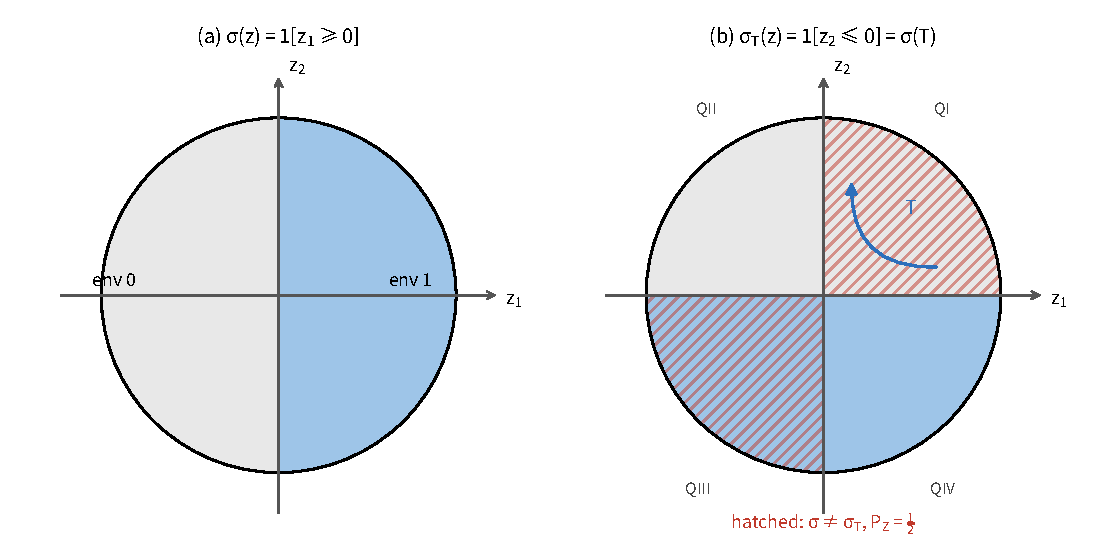
\includegraphics[width=0.92\columnwidth]{fig5_witness.pdf}
\caption{The $d=2$ non-identification witness. Left: the assignment $\sigma=\mathbb 1[z_1\ge0]$ splits the disk by the first coordinate. Right: the rotated assignment $\sigma'=\sigma\circ T=\mathbb 1[z_2\le0]$; the hatched first and third quadrants are where the two disagree, with total probability $1/2$, while the quarter turn leaves the pooled distribution unchanged.}
\label{fig:witness}
\end{figure}

On \(2\times10^5\) draws the disagreement fraction is \(0.5000\), and
the squared maximum-mean-discrepancy between \(Z\) and \(T(Z)\) is
\(0.00058\), finite-sample noise around a population value of zero. This
is a single \(d=2\) witness on the class of arbitrary measurable
assignments, not a claim that every pooled distribution is
non-identifiable, and the witness need not remain inside a smaller
structured class.

The component laws in the witness are not Gaussian. Each environment is
uniform on a half-disk, a bounded-support law with mean
\(4/(3\pi)\approx 0.424\) along the symmetry axis and covariance
approximately \(\mathrm{diag}(0.070,0.250)\). The construction therefore
lives in the broad class of bounded-support models, not the parametric
Gaussian class used later, and the freedom it exploits is freedom in the
component laws themselves, which a fixed parametric family removes.
Classical finite-mixture identifiability, in the form of
Teicher~\cite{teicher1963}, states that a Gaussian
mixture with a known number of distinct components is identifiable up to
a label permutation, so two genuinely different Gaussian partitions with
one pooled law cannot be constructed. That is exactly why the
constrained model in the next section reaches point identification.

A second, covariance-level example illustrates the same limitation
within a Gaussian setting. Consider two zero-mean two-component Gaussian
models with equal weights. In the first the component covariances are
\(\Sigma_1=\mathrm{diag}(1,3)\) and \(\Sigma_2=\mathrm{diag}(3,1)\); in
the second they are \(\Sigma_1'=\Sigma_2'=\mathrm{diag}(2,2)\). Both
induce the same pooled covariance, \(\mathrm{diag}(2,2)\), yet the
component structures differ and the full distributions are not the same.
A single pooled second moment is a many-to-one summary, so it cannot
recover the assignment. The full distribution of a fixed Gaussian family
can, up to permutation, and that distinction is the boundary between the
present witness and the point-identification result that follows.

\subsection{Point identification in a symmetric two-component
covariance-mixture
model}\label{point-identification-in-a-symmetric-two-component-covariance-mixture-model}

Tighten the setting and the decomposition set collapses to a point. Let
\(E\in\{+1,-1\}\) carry equal weight, with zero-mean Gaussian components

\[X\mid E=+1\sim N(0,I+K),\qquad X\mid E=-1\sim N(0,I-K),\]

where \(K\) is symmetric and every eigenvalue of \(K\) lies strictly
inside \((-1,1)\). The pooled covariance is \(I\), so the frame is
whitened. The object identified is the unordered component covariance
pair \(\{I+K,I-K\}\), not the pooled covariance and not any recording
assignment. The result is a special fourth-moment inversion: with the
second moment fixed by whitening, the fourth-order cumulant tensor is
inverted algebraically to recover the pair.

\begin{theorem}[point identification of the component covariance pair]\label{thm:pointid}
In the symmetric two-component model above, the fourth-order cumulant tensor determines $K$ up to the global sign $K\leftrightarrow-K$ in $d=2$, and hence determines the unordered component covariance pair uniquely. Write $K=Q\operatorname{diag}(\lambda_1,\lambda_2)Q^\top$. The following cases are exhaustive.

\textbf{Case (i): $\lambda_1^2\ne\lambda_2^2$.} The contraction $T$ has two distinct eigenvalues, and diagonalizing it recovers the eigenbasis; the eigenvalue magnitudes and their relative sign follow from the diagonal cumulants.

\textbf{Case (ii): $\lambda_1=-\lambda_2\ne0$, so $\operatorname{tr}K=0$ and $T$ is scalar.} The entries of $K$ are recovered directly from the full tensor by the algebraic identities~\eqref{eq:direct-recover}, with no ratio and no singular direction; the swap configuration $K_{11}=0$ is included.

\textbf{Case (iii): $\lambda_1=\lambda_2\ne0$, so $K=\lambda_1 I$ is isotropic.} There is no basis to recover, and the single value follows from $\kappa_{1111}/3$.

\textbf{Case (iv): $\lambda_1=\lambda_2=0$, so $K=0$.} The zero cumulant tensor forces $K=0$ uniquely, but the two component covariances coincide at $I$; two distinct components and an eigenbasis are not identified.

The only genuine observational freedom is the global sign $K\leftrightarrow-K$, which is exactly the label permutation exchanging $I+K$ with $I-K$.
\end{theorem}

\emph{Proof sketch.} The pooled fourth cumulant is
\(\kappa_{ijkl}=K_{ij}K_{kl}+K_{ik}K_{jl}+K_{il}K_{jk}\). Contracting
the middle indices gives a matrix that commutes with \(K\) and, whenever
it is non-scalar, reveals the eigenbasis, after which the diagonal
cumulants fix the magnitudes and the relative sign; the scalar,
isotropic, and zero cases follow from the algebraic
identities~\eqref{eq:direct-recover} and
\(\kappa_{1111}/3\). The full derivation, including the swap
configuration and the sign recovery, is in Appendix A.1.

The same tensor structure appears in higher dimensions, where locating
the eigenbasis is a symmetric tensor decomposition, but we do not prove
that extension and the formal theorem is stated for \(d=2\). The generic
map for centered Gaussian mixtures is non-injective at fourth order and
reaches injectivity at sixth order, as discussed in Chapter 2 and the
finite-moment literature cited there. Whitening, the two-component
restriction, equal weights, and symmetry are the conditions that yield
injectivity, so this is not a generic fourth-order theorem.

The whitening is a population condition. The theorem assumes the pooled
covariance is exactly \(I\), so the whitening is population-known.
Estimating it from a finite sample introduces sampling error and the
cumulant inversion would then be approximate, and a finite-sample
theorem with estimated whitening is not established here. The result is
a population statement on an idealized Gaussian frame and has no direct
applicability to the empirical EEG covariance features, which are
estimated and not whitened in this model.

Two terms should be kept apart. The theorem identifies the unordered
covariance pair, which can collapse to a singleton when \(K=0\), as in
Case (iv); it does not identify two distinct environments in that
degenerate case, which require \(K\ne0\). Neither case identifies
recording-level labels, which lie outside the scope of the theorem.

\subsection{Scope}\label{scope-4}

These results operate on one pooled marginal and identify either the
partition witness or the unordered component parameters. They do not
identify recording assignments, establish finite-sample recovery, or
support the DELVE algorithm in Section 5. No implication runs from one
mechanism to the other, and the generic non-Gaussian, fully blind
identification problem remains open and is stated in the limitations.


\section{Recovery Theory}
\subsection{A recording-level model}\label{a-recording-level-model}

The unit of analysis is the recording, not the window. Write the
transformed recording feature as

\[X_r = A x_r^{(0)} + b \in \mathbb R^p,\qquad Z_r\in\{1,\dots,K\},\]

and define the environment-specific mean, the mixing weight, and the
smallest center separation by

\[\mu_e = E[X\mid Z=e],\qquad \pi_e=P(Z=e),\qquad
\Delta=\min_{e\ne f}\|\mu_e-\mu_f\|.\]

The population K-means risk and its optimum are

\begin{equation}\label{eq:risk}
R(c)=E\!\left[\min_k\|X-c_k\|^2\right],\qquad R^\star=\inf_c R(c).
\end{equation}

\begin{definition}[center space, tie-breaking, and the misclassification rate]\label{def:err}
A center configuration is an ordered $K$-tuple $c=(c_1,\dots,c_K)$ in $(\mathbb R^p)^K$, and configurations that differ only by the relabeling action of the symmetric group $S_K$ are identified in the quotient $(\mathbb R^p)^K/S_K$. The bounded center domain is $\mathcal C_B=(\overline{\mathcal B_p(B)})^K/S_K$. For a configuration $c$, the nearest-center rule is $g_c(x)=\arg\min_k\|x-c_k\|^2$, with ties broken by a fixed measurable rule so that $g_c$ is defined at every point. The misclassification rate is
$$\mathrm{Err}(c,Z)=\min_{\tau\in S_K}P\{g_c(X)\ne\tau(Z)\},$$
which is invariant to label permutation and takes values in $[0,1]$.
\end{definition}

The model is conditional on the feature the pipeline builds,
\(X_r=A[\frac1{W_r}\sum_w\operatorname{vech}\{\log(\widehat\Sigma_{rw})\}]+b\).
Window-level dependence enters the residual, and the recording variance
is governed by the effective window count \(T_{\rm eff}\), not the
nominal \(W_r\). The systematic
Ledoit--Wolf~\cite{ledoit2004} and matrix-log bias
shifts the center, with \(E[\mu_{e,T}]-\mu_e=O(T_{\rm eff}^{-1})\),
while the random fluctuation is noise. The finite-sample theorem treats
\((A,b)\) as a pre-given, deterministic transformation. A StandardScaler
fitted on the data stays random even when frozen afterwards, so it does
not meet this condition. A full-pool scaler belongs to the transductive
variant, and a scaler fitted on the training subset is treated as an
empirical variant.

\subsection{Assumptions}\label{assumptions}

We work with a location model \(X=\mu_Z+\xi_Z\), where
\(E[\xi_e\mid Z=e]=0\).

The assumptions separate into two layers. The first layer,
Assumptions~\ref{a:weights}--\ref{a:sep} together with
the population alignment in Assumption~\ref{a:align},
gives zero-error recovery of the population global minimizer. The second
layer, the closed level sets in
Assumption~\ref{a:closed} and the quadratic growth in
Assumption~\ref{a:growth}, is used only for the positive
risk gap and the quantitative risk-transfer statements; neither is
needed for the zero-error result.

\begin{assumption}[weights]\label{a:weights}
$\pi_e\ge\pi_{\min}>0$ for every $e$.
\end{assumption}

\begin{assumption}[concentration, hard ball]\label{a:conc}
$\|\xi_e\|\le\rho$ almost surely.
\end{assumption}

\begin{assumption}[separation]\label{a:sep}
$\Delta>4\rho$.
\end{assumption}

The hard-ball and separation assumptions define an idealized benchmark,
not the empirical setting of this paper. They are geometric premises
used to state the conditional transfer cleanly, and they are not
satisfied by Gaussian or sub-Gaussian residuals, whose support is
unbounded, or by the EEG covariance features. The experiments do not
claim otherwise. The next section lifts them to unbounded sub-Gaussian
tails through a high-probability argument.

For a point from environment \(e\), its distance to its own center is at
most \(\rho\), while \(\|X-\mu_f\|\ge\Delta-\rho>3\rho>\|X-\mu_e\|\) for
\(f\ne e\). This gives the next lemma.

\begin{lemma}[the true-center classifier is correct]\label{lem:truecenter}
Under Assumptions~\ref{a:weights}--\ref{a:sep}, the nearest-center classifier at the true centers satisfies $g_\mu(X)=Z$ almost surely.
\end{lemma}

The lemma says only that the true centers classify correctly; it does
not say they solve the population K-means problem.

\begin{assumption}[population K-means alignment]\label{a:align}
For fixed $K$ and a pre-given transformation, every global minimizer of the population K-means risk assigns exactly one center to each environment:
$$\mathcal C^\star=\{c:R(c)=R^\star\}=\{(\mu_1,\dots,\mu_K)\text{ up to label permutation}\}.$$
The set $\mathcal C^\star$ is the optimizer set within the bounded domain $\mathcal C_B$, not an unconstrained full-space minimizer; the radius $B$ is taken large enough that every environment mean lies in $\overline{\mathcal B_p(B)}$.
\end{assumption}

This is a direct condition on the geometry of the population objective,
not a consequence of any split or merge calculation, and it is stronger
than pairwise mean separation. It identifies the entire global optimizer
set, not merely the correctness of the nearest-mean classifier.

\begin{lemma}[boundary-tube vanishing on a non-degenerate center domain]\label{lem:closed}
In the bounded frame $\|X\|\le B$ with the law of $X$ absolutely continuous, on the non-degenerate domain $\mathcal C_{B,d_{\min}}$ where distinct centers stay at least $d_{\min}$ apart, $\mathrm{Err}(c,Z)$ is continuous and every level set is closed.
\end{lemma}

\begin{assumption}[closed level sets]\label{a:closed}
The misclassification function $\mathrm{Err}(c,Z)$ is upper semicontinuous on the center domain; equivalently, every level set $\mathcal C_q=\{c:\mathrm{Err}(c,Z)\ge q\}$ is closed. On the non-degenerate domain this follows from Lemma~\ref{lem:closed}; on the full domain, including coincident centers, it is retained as an explicit assumption.
\end{assumption}

The lemma does not cover coincident centers, where an arbitrarily small
perturbation can place the new bisector through a region of positive
probability; the one-dimensional counterexample is given in Appendix
A.5.

\begin{assumption}[quadratic growth]\label{a:growth}
$R(c)-R^\star\ge\kappa_0\,d(c,\mathcal C^\star)^2$, where $d(c,\mathcal C^\star)=\min_{\pi\in S_K}\big(\sum_k\|c_k-\mu_{\pi(k)}\|^2\big)^{1/2}$ is the distance on the quotient $\mathcal C_B$, minimized over label permutations. The constant $\kappa_0$ is distinct from the fourth-order cumulant $\kappa_{ijkl}$ used in Chapter 4.
\end{assumption}

This is an independent strong assumption. The margin condition does not
imply it, and the quantitative bound it supports is local. The split and
merge quantities used in the diagnostics are reported as descriptive
only; they do not establish population optimality, and the local
exchange argument built on them has been withdrawn.

\subsection{The conditional compatibility
theorem}\label{the-conditional-compatibility-theorem}

The recording-level guarantee follows a fixed route: population
alignment identifies the optimal centers, a positive risk gap converts
excess risk into a label-error bound, and uniform control of the
empirical risk turns that into a finite-sample statement. The theorem is
conditional on the population K-means alignment above, which fixes the
whole global optimizer set rather than only the nearest-mean decision
rule; it is not an identification result derived from the generative
model.

\begin{theorem}[conditional population recovery under K-means alignment]\label{thm:A}
Suppose Assumptions~\ref{a:weights}--\ref{a:sep} and Assumption~\ref{a:align} hold. Then for some permutation $\pi$,
$$P\{g_{c^\star}(X)\ne\pi(Z)\}=0.$$
\end{theorem}

\emph{Proof sketch.} Assumption~\ref{a:align} identifies
the optimal centers as a permutation of the means, which
Lemma~\ref{lem:truecenter} makes error-free. The full
proof is in Appendix A.3.

The recovery comes from the alignment that is assumed, not from a
lower-level generative argument. The Conditional Compatibility Theorem
states that K-means compatibility implies risk-gap recovery; it is not a
generative bridge from recording separation to partition recovery.

For a target misclassification level \(q\), set

\begin{equation}\label{eq:margin}
\mathcal C_q=\{c:\mathrm{Err}(c,Z)\ge q\},\qquad
\psi(q)=\inf_{c\in\mathcal C_q}\{R(c)-R^\star\}.
\end{equation}

\begin{lemma}[compact center domain and continuity of the risk]\label{lem:compact}
In the bounded-feature frame $\|X\|\le B$, the center space $\mathcal C_B$ is compact, the population risk $R$ is continuous on it, and an optimizer can be taken inside $\mathcal C_B$.
\end{lemma}

\begin{theorem}[positive risk gap]\label{thm:B}
Under the assumptions of Theorem~\ref{thm:A} together with Assumption~\ref{a:closed}, for every $q>0$ with $\mathcal C_q\ne\varnothing$,
\begin{equation}\label{eq:compatibility}
\psi(q)>0.
\end{equation}
\end{theorem}

\emph{Proof sketch.} The optimal set has error zero, so the closed level
set \(\mathcal C_q\) excludes it. Compactness and continuity then force
the infimum of \(R-R^\star\) to be attained and strictly positive. The
full proof is in Appendix A.3.

A quantitative form is available only locally. Let the margin obey
\(P(X\in\mathcal M_t)\le C_{\rm margin}t^\beta\), with \(\beta=1\) in
the ordinary case. Inside the local stability region, combining the
margin relation with Assumption~\ref{a:growth} gives

\[\psi(q)\ge\kappa_0\Big(\frac{q}{C_{\rm margin}}\Big)^{2/\beta}\quad\text{for }0<q\le q_0.\]

For \(\beta=1\), \(\psi(q)\ge(\kappa_0/C_{\rm margin}^2)q^2\). The
cutoff \(q_0\) is the largest level at which the local linearization
holds. We claim no global quantitative bound, and neither \(\kappa_0\)
nor \(C_{\rm margin}\) is self-certified.

\subsection{Finite-sample transfer}\label{finite-sample-transfer}

Let \(\widehat R_M\) be the empirical risk on \(M\) independent
recordings, let
\(\varepsilon_M=\sup_{c\in\mathcal C}|\widehat R_M(c)-R(c)|\), and let
\(\delta_{\rm opt}=\widehat R_M(\widehat c)-\widehat R_M^\star\) be the
optimization error. The standard excess-risk decomposition is

\begin{equation}\label{eq:risk-gap}
R(\widehat c)-R^\star\le 2\varepsilon_M+\delta_{\rm opt}.
\end{equation}

\begin{lemma}[risk transfer]\label{lem:transfer}
Fix $q>0$ with the level set $\mathcal C_q$ closed so that $\psi(q)$ is well defined. For any configuration $\widehat c$,
$$R(\widehat c)-R^\star<\psi(q)\quad\Longrightarrow\quad \mathrm{Err}(\widehat c,Z)<q.$$
Combined with the excess-risk decomposition, $2\varepsilon_M+\delta_{\rm opt}<\psi(q)$ implies $\mathrm{Err}(\widehat c,Z)<q$.
\end{lemma}

The implication is conditional: it does not assume alignment and does
not assert that \(\psi(q)\) is positive. For bounded features, the
uniform deviation admits an explicit grid bound. An \(\eta\)-net of the
stacked center domain has size \(N_\eta\le(1+2\sqrt K B/\eta)^{Kp}\),
and the cell function is \(4B\)-Lipschitz in the product center norm. A
Hoeffding bound and a union over the net give, with probability at least
\(1-\alpha\),

\[\varepsilon_M\le h(M,\eta),\qquad
h(M,\eta)=\sqrt{\frac{8B^4\log(2N_\eta/\alpha)}{M}}+8B\eta.\]

The covering, Lipschitz, and Hoeffding derivation is in Appendix A.4.

\begin{corollary}[nontrivial finite-sample recovery]\label{cor:finite}
Suppose every assumption of Theorem~\ref{thm:B} holds and choose $q$ with $\psi(q)>0$. For a global empirical minimizer, $\delta_{\rm opt}=0$, and if
$$2h(M,\eta)<\psi(q),$$
then with probability at least $1-\alpha$, $\mathrm{Err}(\widehat c,Z)<q$. For a finite-initialization Lloyd solution the same conclusion holds with probability at least $1-\alpha$ under $2h(M,\eta)+\delta_{\rm opt}<\psi(q)$.
\end{corollary}

\emph{Proof sketch.} On the event \(\varepsilon_M\le h(M,\eta)\), the
excess-risk decomposition gives excess risk below \(\psi(q)\), and the
risk-transfer lemma then yields \(\mathrm{Err}(\widehat c,Z)<q\). The
positivity \(\psi(q)>0\) is the content of
Theorem~\ref{thm:B}; without it the bound is the empty
conditional.

\subsubsection{High-probability sub-Gaussian
truncation}\label{high-probability-sub-gaussian-truncation}

The hard-ball radius is a deterministic support bound. A sub-Gaussian
tail replaces it with a radius that holds with a chosen probability,
with no bounded-support requirement.

\begin{assumption}[sub-Gaussian residuals]\label{a:sg}
There is a constant $\sigma\ge 0$ such that, for every environment $e$ and every $v\in\mathbb R^p$, $\|\langle v,\xi_e\rangle\|_{\psi_2}\le \sigma\|v\|$. Here $\|Y\|_{\psi_2}=\inf\{t>0:E[\exp(Y^2/t^2)]\le 2\}$ is the sub-Gaussian Orlicz norm.
\end{assumption}

For a sub-Gaussian vector in \(\mathbb R^p\), there are universal
constants \(C_1,c_2>0\) such that
\[P\big(\|\xi_e\|>C_1\sigma(\sqrt p+t)\big)\le 2\exp(-c_2t^2/\sigma^2).\]
For \(\delta\in(0,1)\), define the high-probability radius
\[\rho_\delta=C\sigma\sqrt{p+\log(K/\delta)},\] where \(C\) is
universal. A union bound over the \(K\) environments gives
\[P\big(\max_e\|\xi_e\|>\rho_\delta\big)\le\delta.\]

\begin{proposition}[conditional lift under truncation]\label{prop:trunc}
Let $E_\delta=\{\max_e\|\xi_e\|\le\rho_\delta\}$. On $E_\delta$, which has probability at least $1-\delta$, the hard-ball assumptions hold with $\rho$ replaced by $\rho_\delta$. If $\Delta>4\rho_\delta$ and the population alignment in Assumption~\ref{a:align} holds on the truncated population, the zero-error classification, the conditional recovery of Theorem~\ref{thm:A}, and the finite-sample Corollary~\ref{cor:finite} carry over, conditioned on $E_\delta$, with $\rho_\delta$ in place of $\rho$.
\end{proposition}

For a finite sample of \(M\) independent recordings, the union bound is
over the \(M\) observations and the radius becomes
\(\rho_{\delta,M}=C\sigma\sqrt{p+\log(KM/\delta)}\), with the same
probability and the same conditional conclusion.

Three qualifications are part of the statement. First, truncation
relaxes the support condition only; the population alignment remains an
explicit premise, and the proposition does not derive it. Second, the
radius and the required separation grow as \(\sqrt{\log(1/\delta)}\), so
higher confidence demands a larger separation, the cost of unbounded
support. Third, outside \(E_\delta\), an event of probability at most
\(\delta\), the hard-ball conclusion is not asserted; with a bounded
loss the unconditional statement adds a term of order \(\delta\).

\subsection{The DELVE procedure and operational
variants}\label{the-delve-procedure-and-operational-variants}

The estimand and the guarantee are operationalized by one procedure,
listed in Algorithm~\ref{alg:delve}. The bracketed tags
separate standard components from this paper's estimand and guarantee.

\begin{algorithm}[H]
\centering
\small
\renewcommand{\arraystretch}{1.15}
\begin{tabular}{@{}r >{\raggedright\arraybackslash}p{0.78\columnwidth}@{}}
\textbf{Input} & recordings $\{R_1,\dots,R_M\}$, grid $\mathcal K=\{2,\dots,6\}$, level $\alpha$\\
\textbf{Output} & $\hat K$, hard labels $\hat\ell_r$, soft posteriors $\eta_{rk}$, stability, bootstrap, sensitivity\\
\textbf{Stage 0} & [standard] homogenize: shared channels, common-average reference, band-pass with notch, resample, four-second windows\\
\textbf{Stage 1} & [standard] per window $\widehat\Sigma_w=\mathrm{LedoitWolf}$; $x_w=\operatorname{vech}(\log\widehat\Sigma_w)$\\
\textbf{Stage 2} & [this paper's estimand] $x_r=\frac1{W_r}\sum_w x_w$; $X=\mathrm{StandardScaler}$ across recordings\\
\textbf{Stage 3} & [standard] K-means fitting followed by nearest-centroid assignment; BIC, silhouette, and stability score; $\hat K$\\
\textbf{Stage 4} & [theoretical guarantee, not a computed output] the conditional misclassification statement of Corollary~\ref{cor:finite}; its terms are population quantities, and the procedure evaluates no numeric bound\\
\textbf{Stage 5} & [standard] co-assignment and resampling stability\\
\textbf{Stage 6} & [standard] assignment bootstrap and perturbation sensitivity\\
\textbf{Stage 7} & post-hoc interpretation using metadata, not an algorithm output\\
\end{tabular}
\caption{The DELVE procedure for recording-level environment recovery. The standard components (Stages 0--1, 3, 5--6) are not claimed as novel; the contribution lies in the unified recording-level estimand (Stage 2) and the conditional misclassification guarantee (Stage 4). Automatic $K$ selection and the full-pool scaler stay outside the unconditional guarantees.}
\label{alg:delve}
\end{algorithm}

The same staged flow is shown as a diagram in
Figure~\ref{fig:pipeline}.

\begin{figure}[htbp]
\centering
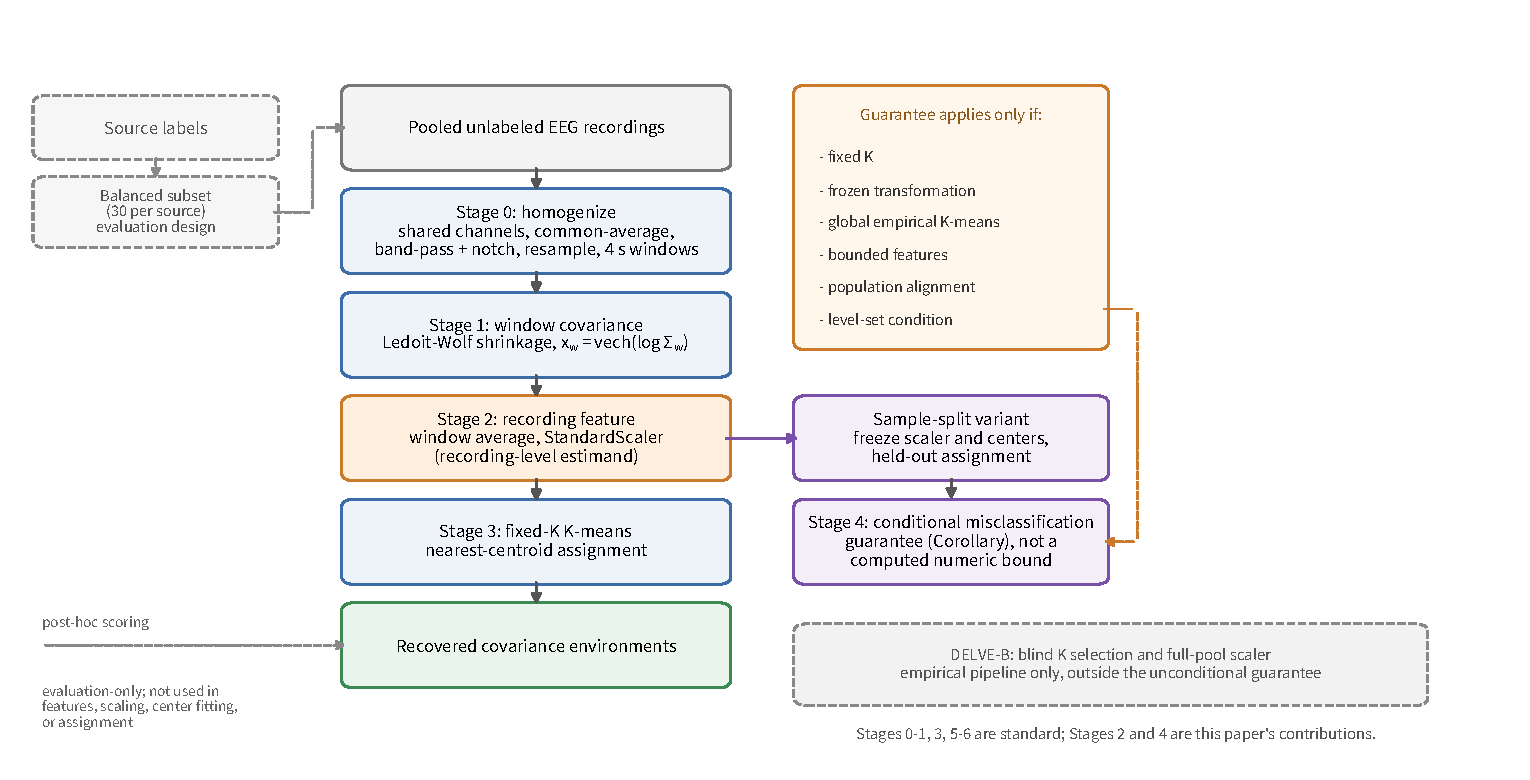
\includegraphics[width=0.74\columnwidth]{fig6_pipeline.pdf}
\caption{Core DELVE processing pipeline and evaluation-only label usage. The staged core runs from pooled unlabeled EEG to recovered covariance environments; the recording-level estimand (Stage 2) is highlighted, and the sample-split branch leads to the Stage 4 conditional misclassification guarantee, a theoretical statement, not a computed numeric bound. The source labels (dashed) are used only to construct the prespecified balanced evaluation subset, thirty recordings per source, and for post-hoc scoring; they are not used to construct features, fit the scaler, select centers, or assign clusters. The remaining stages are standard components.}
\label{fig:pipeline}
\end{figure}

The two-way sample-split fits the scaler and centers on one half and
freezes them for the held-out half. Because the scaler and centers share
the same training data, this is an empirical inductive variant, not the
conditional theorem. A strict three-way split separates the scaler,
center, and evaluation recordings, so the scaler is independent of the
center fit and the held-out assignment; we report it as an inductive
empirical check. The three operational variants, fully compared in
Supplementary Table S6, are DELVE-G, which fixes \(K\) and uses a
pre-given transformation and a global minimizer with zero optimization
error and is covered in full by the risk-gap guarantee; DELVE-L, which
keeps fixed \(K\) but uses finite-initialization Lloyd and carries the
explicit \(\delta_{\rm opt}\); and DELVE-B, the blind pipeline with a
data-dependent scaler and a prespecified selector, which carries no
unconditional guarantee.

Freezing a fitted scaler does not make it pre-given. The guarantee
attaches to the global empirical K-means solution under fixed \(K\), a
pre-given transformation, bounded features, and the alignment and
level-set assumptions. Automatic \(K\) selection, data-dependent
standardization, and finite-initialization Lloyd fall outside it, and
the paper does not establish that the unlabeled EEG satisfies the
conditions. Proving alignment on a structured distribution class through
a capture or exchange argument is left as future work.


\section{Synthetic and Semi-synthetic Experiments}
\subsection{Experimental setup and population
reference}\label{experimental-setup-and-population-reference}

The theory states an implication. Under alignment and closed level sets,
a positive risk gap separates the global empirical solution from
configurations that misclassify, and a solution whose excess risk stays
below the gap inherits the misclassification bound. Controlled
experiments can diagnose whether the implication is consistent with the
premises on a large reference sample and show what happens when the
premises fail; they cannot establish the population conditions or
generate the alignment premise.

The main design is a Gaussian location model with three environments,
ten feature dimensions, equal weights, and unit noise. Three centers sit
on an equilateral geometry in the first two coordinates, and the
signal-to-noise ratio sets the spacing. A reference sample of \(10^5\)
draws serves two purposes. It gives a finite-reference diagnostic of
population alignment by comparing the optimal three-center and
two-center empirical risks, instead of assuming the former, and it
estimates the reference risk-gap curve \(\widehat\psi_{\rm ref}(q)\)
through center perturbation.

The perturbation diagnostic uses a fixed candidate set, not the full
center space. Twenty perturbation radii from zero to five are crossed
with sixteen random unit directions in the ten-dimensional space, giving
three hundred and twenty candidate configurations. The curve
\(\widehat\psi_{\rm ref}(q)\) is the smallest risk difference among the
candidates whose misclassification reaches \(q\). It is a finite
candidate-set minimum, not the population infimum, and it carries no
guarantee of reaching the population value in
Corollary~\ref{cor:finite}. The alignment diagnostic has
the same status.

Two signal-to-noise settings are used, six and nine tenths. The SNR-six
geometry is examined under both Gaussian and bounded-uniform noise, and
the nine-tenths setting matches the order of the separation measured on
the real EEG, which makes it the relevant negative control, not a straw
case.

\subsection{The Gaussian robustness arm and the bounded-noise
theorem-compatible
arm}\label{the-gaussian-robustness-arm-and-the-bounded-noise-theorem-compatible-arm}

The first arm, the Gaussian robustness arm, uses signal-to-noise ratio
six, where the alignment and level-set conditions are empirically
diagnosed on the reference, not assumed. The true centers misclassify
about three points in a thousand, and the two-center optimum runs
roughly six units above the three-center optimum. The estimated gap
curve is positive at every target level, rising from about \(6.7\) at
\(q=0.05\) to about \(15.7\) at \(q=0.20\).

One premise is not met by this design. Gaussian noise has unbounded
support, so no finite \(\rho\) makes the almost-sure hard-ball condition
hold; the reference shows an empirical truncation, not the
probability-one condition, and the alignment and level-set premises are
finite-reference diagnostics as well. The observed pattern is consistent
with the risk-gap implication with no violation, but the theorem as a
whole does not apply because the hard-ball premise fails, and the
population quantities are only estimated. We read this arm as an
empirical robustness study under model misspecification.

Across the finite-sample sweep, sixty independent repetitions are drawn
at each sample size, and the global empirical solution is scored on the
held-out reference. Excess risk falls from about \(2.35\) at the
smallest size to under one tenth at the largest, and misclassification
falls with it, from about nine per thousand to three. Whenever the
excess sits below the gap for a level, the error stays below that level,
with no violation in any repetition. The misclassification displays a
sharp phase transition consistent with the risk-gap implication, but it
does not validate the theorem because the gap is reference-estimated.
Figure~\ref{fig:sweep} plots the sweep against the
reference-estimated gap thresholds and the target levels.

\begin{figure}[htbp]
\centering
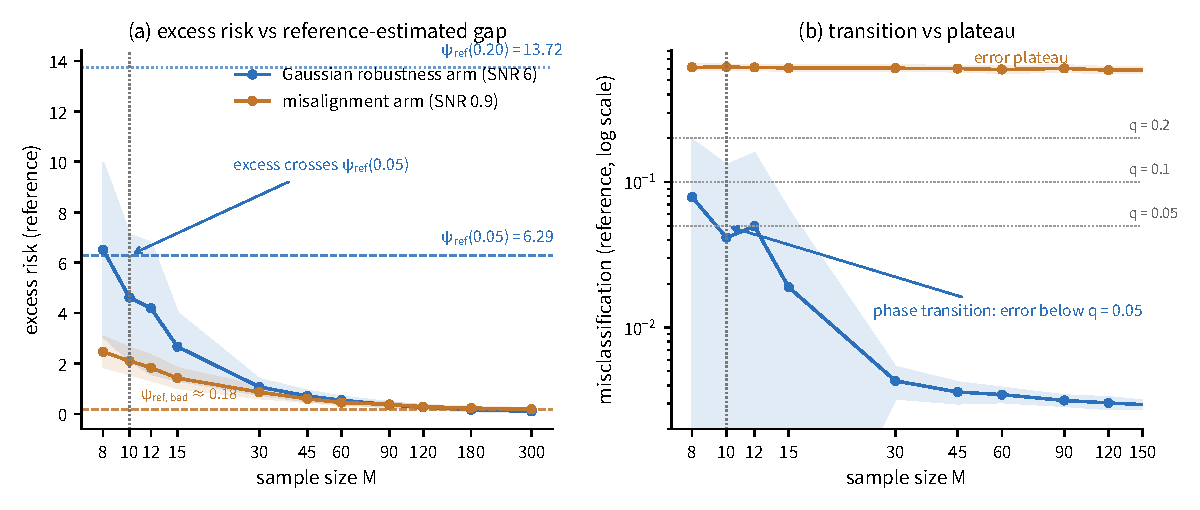
\includegraphics[width=\textwidth]{fig7_ch6_sweep.pdf}
\caption{Finite-sample sweep over sixty repetitions. Left: excess risk against sample size with the reference-estimated gap thresholds $\widehat\psi_{\rm ref}(0.05)$ and $\widehat\psi_{\rm ref}(0.20)$; the excess crosses $\widehat\psi_{\rm ref}(0.05)$ near $M=10$. These are reference-sample diagnostic thresholds, not population quantities. Right (log scale): misclassification falls below $q=0.05$ after the crossing for the aligned arm, while the negative control stays on a plateau near $0.6$. The Gaussian arm is a robustness experiment because the hard-ball assumption fails; the bounded-uniform arm is the only arm whose support condition holds analytically.}
\label{fig:sweep}
\end{figure}

The hard-ball premise deserves a design that satisfies it rather than
approximating it. The second arm, the bounded-noise theorem-compatible
arm, keeps the same geometry but replaces the Gaussian noise with
isotropic noise uniform on a ball of radius \(\rho\). The hard-ball
condition then holds almost surely by construction, and the equilateral
spacing is set to \(\Delta=6\rho\), which strictly exceeds the \(4\rho\)
the margin requires. On the reference, the empirical maximum noise norm
is exactly \(\rho\), and the nearest-center classifier at the true
centers makes no error at all. The finite-sample sweep repeats the same
fit across the same sizes and sixty repetitions: excess risk falls from
about \(0.19\) to under one hundredth, misclassification stays at zero,
and the gap implication has no violation.

The premises do not all have the same logical status. The hard-ball
support and the margin hold analytically and with probability one, while
the population alignment and the gap curve are finite-reference
diagnostics. The reference therefore gives a numerical diagnosis of the
theorem's chain, not a proof of it, and a larger reference would only
sharpen the estimate.

Three secondary robustness checks sharpen the boundary without
standalone tables. With the shape left free, the pooled fourth moment
stays non-identified as each higher moment introduces a new shape
parameter, and jointly estimating the shape does not converge in the
tested Student-\(t\) design. A median-of-means robust variant is more
stable in the specified Huber and heavy-tailed configurations, but the
non-asymptotic bound weakens as the environments approach each other. A
pre-specified grid sweep shows that underestimating \(K\) merges the
same pair while overestimating adds nested refinement with no elbow,
which supports keeping automatic selection outside the guarantees.

\subsection{The misalignment arm (negative
control)}\label{the-misalignment-arm-negative-control}

At signal-to-noise ratio nine tenths the picture changes. The true
centers misclassify close to half the reference, and the
two-versus-three-center gap shrinks to about half a unit, with the
estimated gap curve near zero. The empirical excess still declines as
the sample grows, from about \(1.48\) to under one fifth, yet
misclassification does not follow. It stays on a plateau near sixty
percent with no phase transition across the whole sweep.

That plateau is the informative result. When the population optimum is
not aligned with the true labels, adding data cannot restore them,
because the object being estimated is itself misaligned. A mechanical
count of gap violations is not meaningful here, since the gap is near
zero and its reference estimate carries finite-sample noise. We read the
arm through its one stable fact, the error plateau, and we do not report
noisy threshold crossings as counterexamples. The arm parallels the real
EEG, whose separation is of the same order and whose recovery numbers
are diagnostic, not validation.

\subsection{Summary}\label{summary-6}

The experiments establish four facts. On the Gaussian arm, where the
hard-ball support fails, the pattern stays consistent with the risk-gap
implication with no violations and a clear phase transition, an
empirical robustness result, not validation. The bounded-noise design
meets the hard-ball premise and margin analytically, while its alignment
and gap curve remain finite-reference diagnostics; it classifies with
zero error and zero violations but does not validate the chain. When the
optimum is misaligned, more data leave a stable error plateau, and the
same holds under unknown non-Gaussian shapes. The compatibility premise
stays an assumption throughout.


\section{Recording-level Covariance Clustering Across EEG Sources}
\subsection{Three independent sources and one
protocol}\label{three-independent-sources-and-one-protocol}

The empirical study uses three independently collected EEG sources. They
span a wide spread of acquisition and protocol differences, so the
recovered label is interpreted only as a source-associated technical
mixture, and no claim is made that a single device or task can be
isolated as the cause.

The first source is a research-grade BrainVision study with eight
channels at a thousand hertz, thirty-two subjects and sixty-four
recordings. The second is a consumer-grade Emotiv headset with fourteen
channels at a hundred and twenty-eight hertz, thirty subjects and thirty
long recordings. The third is the eyes-open baseline run R01 of the
PhysioNet \emph{EEG Motor Movement/Imagery Dataset} (eegmmidb), a
hundred and nine subjects and sixty-four channels.

All three are reduced to one pre-specified pipeline before any
clustering. Four shared channels are retained, F3, F4, O1, and O2; the
data are resampled to a hundred and twenty-eight hertz, common-average
referenced, band-passed from one to forty hertz with a fifty-hertz
notch, and cut into four-second windows. Window covariances use
Ledoit--Wolf shrinkage and are linearized through the matrix logarithm,
and the recording feature is the unweighted within-recording average.
The protocol is fixed before analysis, and each recording receives one
equal vote. The source-level facts are stated in
Table~\ref{tab:sources}; the complete data processing,
versions, links, and call parameters are in Supplementary S1.

\begin{table}[htbp]
\centering
\small
\caption{The three independently collected EEG sources and their acquisition characteristics. The harmonized pipeline reduces these heterogeneous sources to a common feature space.}
\label{tab:sources}
\begin{tabular}{lllll}
\hline
source (accession) & device & channels & rate & subjects/recordings\\
\hline
ds007541 & BrainVision & 8 & 1000 Hz & 32 / 64\\
ds008099 & Emotiv EPOC & 14 & 128 Hz & 30 / 30\\
on004362 & PhysioNet R01 & 64 & 160 Hz & 109 / 109\\
\hline
\end{tabular}

\end{table}

The recording is the unit of feature construction and of the primary
clustering. Windows estimate a recording's feature and never carry their
own p-values. A separate analysis treats the subject as the independent
unit. All permutation tests use a one-sided upper tail with the plus-one
correction, \(p=(1+\#\{b:T_b\ge T_{\rm obs}\})/(B+1)\), and the smallest
reportable value is \(1/(B+1)\). Each p-value is labeled with its
resampling count and its unit.

The analyses separate into a primary set and a secondary exploratory
set. The primary set is the balanced oracle-\(K\) recovery, the blind
\(K\) selection, the unbalanced full-pool fit, and the subject-level
aggregation, all on the covariance features with the recording as the
unit unless stated. The secondary set in Section 7.5 covers alternative
spatial representations, channel-drop checks, novelty detection,
non-covariance phase locking, and component ablations. No prespecified
multiple-comparison strategy is applied across these analyses, and the
permutation \(p\)-values, ARI figures, and bootstrap intervals are
descriptive diagnostics, not confirmatory hypothesis tests with a
family-wise error guarantee.

Before the clustering results, one caveat frames what a recovered label
can mean. The source labels are fully predictable from recording
metadata alone, the window count ranges having no overlap across the
three sources, so the partition the method recovers is a technical
source-associated structure, not a latent biological environment. The
detailed controls and the feature-to-metadata correlations are in
Section 7.2.

\subsection{Metadata controls}\label{metadata-controls}

A direct diagnostic asks whether the sources are already separated by
information unrelated to latent environments. The number of windows is
nine for every recording in the first source, fifteen in the third, and
ranges from eighty to a hundred and fourteen in the second; the three
ranges do not overlap. A decision tree given only this field predicts
the source with perfect cross-validated accuracy. Subject-grouped folds,
which keep every recording of one subject in a single fold across the
171 subject groups, also give accuracy one, so the result is not
produced by related recordings crossing between folds. Adding the device
metadata constant within a source holds the accuracy at one for both
logistic and tree models. The sources are therefore fully separable from
trivial metadata alone, the clearest evidence that the recovered label
is a technical one.

The association with metadata is quantified rather than asserted. Across
the ten covariance features, the absolute correlation with window count
reaches \(0.663\) and averages \(0.210\). A length-matched control would
be natural, but the data do not permit one. The three window-count
ranges have no common support, and trimming to an overlap would leave an
empty design. We state this as an infeasibility rather than replace it
with a different control.

Two controls check where the structure appears. The same-device control
pools recordings within one source and repeats the clustering there. The
silhouette stays low, between \(0.18\) and \(0.22\), and the clustering
agrees with the subject label at an ARI of only \(0.02\) to \(0.03\), so
no stable within-device structure is recovered. The same-task control
keeps the two resting sources and drops the third; despite the shared
task they still separate at two clusters, with a balanced ARI of
\(0.53\), \(0.56\) over three seeds. A shared task category is therefore
not sufficient to remove the source difference, but the controls cannot
name a single driver because device, population, length, reference, and
preprocessing still differ together. The full metadata table is in
Supplementary S3.

\subsection{Recovery under a known number and blind
selection}\label{recovery-under-a-known-number-and-blind-selection}

\begin{figure}[htbp]
\centering
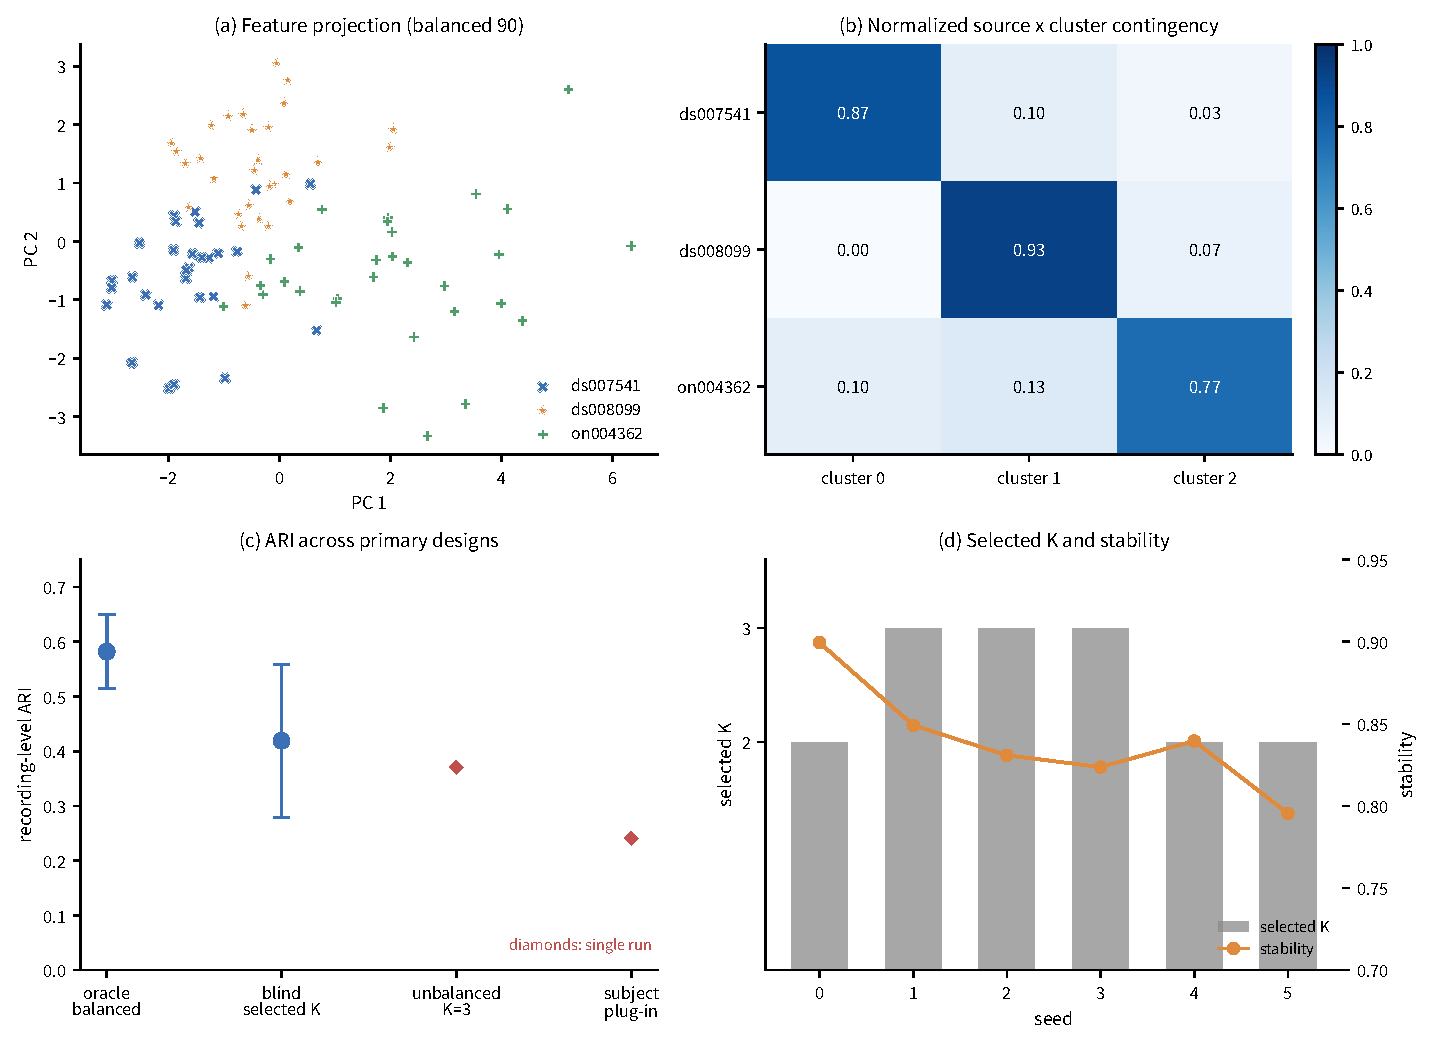
\includegraphics[width=\textwidth]{fig8_main_results.pdf}
\caption{Four-panel main EEG result. (a) Two-dimensional PCA projection of the balanced ninety-recording features, colored by source. (b) Source x cluster contingency at the oracle value $K=3$, normalized within each source, with the diagonal dominant. (c) Recording-level ARI across the four primary designs, with mean and standard deviation for the multi-seed designs and diamonds for single-run realizations. (d) Blind selector: selected $K$ (bars) and bootstrap stability (line) across six balanced seeds. The figure consolidates evidence otherwise spread across the tables and the supplementary.}
\label{fig:main}
\end{figure}

The clearest positive evidence comes from the balanced cross-source
design. With only two sources pooled, every paired combination is
recovered, with ARI between \(0.48\) and \(0.64\). Pooling all three
sources at the oracle value of three strengthens the result. On the
balanced ninety-recording design, recording-level ARI reaches \(0.608\),
and the result holds across six balanced seeds at a mean of \(0.582\),
as detailed in Table~\ref{tab:perseed}.

\begin{table}[htbp]
\centering
\small
\caption{Per-seed recording-level ARI on the ninety-recording balanced design and on the cross-fitted held-out construction, with the sample mean and standard deviation reported rather than a mean alone. The cross-fitted column is defined in Supplementary S1.}
\label{tab:perseed}
\begin{tabular}{lcc}
\hline
seed & balanced $K=3$ ARI & cross-fitted $K=3$ ARI\\
\hline
0 & 0.608 & 0.602\\
1 & 0.589 & 0.630\\
2 & 0.476 & 0.602\\
3 & 0.535 & 0.717\\
4 & 0.607 & 0.617\\
5 & 0.675 & 0.493\\
\hline
mean & 0.582 & 0.610\\
std & 0.068 & 0.072\\
\hline
\end{tabular}

\end{table}

The balanced design is not a blind run. Thirty recordings are drawn from
each source, and the source label is used only to select the recordings;
it never enters the covariance features, the scaler, or the clustering.
The draw and the rule are fixed in advance, so this is a pre-specified
evaluation. It is recording-level, oracle-\(K\) evidence that the source
label can be reconstructed from the covariance features, not an external
validation of the blind pipeline and not a subject-level claim.

The prespecified blind selector does not reproduce the oracle result. On
the seed-0 balanced design it returns two clusters rather than three,
with ARI \(0.279\). Run across all six balanced seeds, the automatic
choice is not fixed: it selects \(K=2\) in three seeds and \(K=3\) in
the other three, and the ARI measured at the selected \(K\) averages
\(0.419\pm0.140\). What stays systematic is the two-cluster geometry.
Whenever \(K=2\) is fitted, the same two sources, ds007541 and ds008099,
are joined, while on004362 stays apart, and the merged cluster separates
cleanly into the two true components once the correct number is
restored. The forced two-cluster ARI averages \(0.277\pm0.043\) across
the seeds. The stability gate drives the under-selection, not the BIC
term, which on its own prefers the larger values, and no prespecified
rule recovers the oracle number on every seed. We present this as a
primary finding rather than a caveat. Covariance structure can be
recoverable at a fixed \(K\) while the number of sources is itself not
reliably selected by the blind procedure. The \(K\) sensitivity across
the full grid is shown in Figure~\ref{fig:ksens}, and
the per-seed numbers are in Table~\ref{tab:blind}.

\begin{table}[htbp]
\centering
\small
\caption{Per-seed blind selection on the balanced ninety-recording design. Each balanced seed uses a fresh \texttt{default\_rng(2026)} for the clustering randomness. The automatic choice is unstable, two clusters in three seeds and three in the other three, but forcing two clusters always merges the same pair, ds007541 and ds008099, with on004362 kept mostly apart. Stability is the bootstrap cluster-agreement at the selected $K$. Alternative RNG constructions retain the same pattern and never select $K=3$ in all six seeds.}
\label{tab:blind}
\begin{tabular}{ccccc}
\hline
seed & selected $K$ & ARI at selected $K$ & forced $K=2$ ARI & stability\\
\hline
0 & 2 & 0.279 & 0.279 & 0.899\\
1 & 3 & 0.589 & 0.326 & 0.849\\
2 & 3 & 0.476 & 0.225 & 0.831\\
3 & 3 & 0.561 & 0.225 & 0.824\\
4 & 2 & 0.296 & 0.296 & 0.840\\
5 & 2 & 0.313 & 0.313 & 0.795\\
\hline
\end{tabular}

\end{table}

\begin{figure}[htbp]
\centering
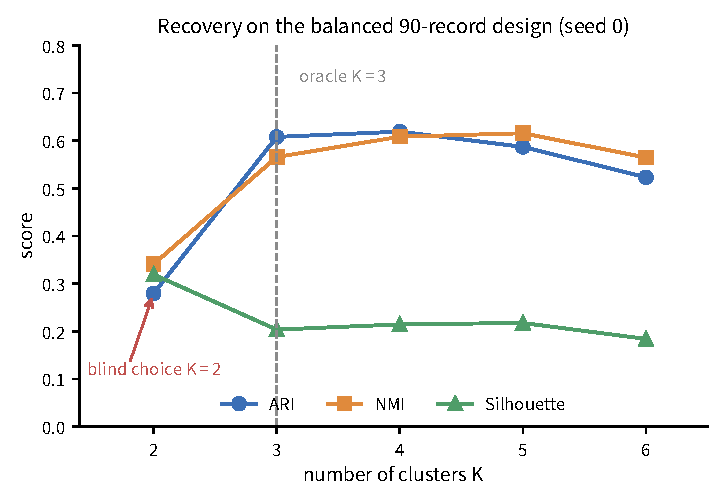
\includegraphics[width=0.85\columnwidth]{fig1_k_sensitivity.pdf}
\caption{This figure compares candidate-$K$ diagnostics with the prespecified oracle evaluation value $K=3$; it does not establish that $K=3$ is identifiable from the pooled data. The adjusted Rand index, normalized mutual information, and silhouette are reported across $K=2,\dots,6$ on the balanced ninety-recording design. The blind selector stops at two clusters with ARI $0.279$, the oracle value of three gives $0.608$, and the scores plateau before declining as extra clusters split the sources.}
\label{fig:ksens}
\end{figure}

\subsection{Balance and subject-level
uncertainty}\label{balance-and-subject-level-uncertainty}

The balanced design does real work, and removing it lowers the point
estimate. On the full unbalanced pool the recording-level ARI falls to
\(0.371\). The most direct plug-in, run once over all subjects without
resampling, is weaker still. With a hundred and seventy-one subjects in
unequal group sizes, the subject-level ARI is only \(0.241\). The large
source is split across several clusters and the small sources merge, the
same mechanism seen in the unbalanced recording result. Balance is
therefore a condition for recovery, not a cosmetic detail. The four
primary designs are consolidated in
Table~\ref{tab:designs}.

\begin{table}[htbp]
\centering
\small
\caption{ARI across the four primary designs, with the statistical scope stated for each row. The balanced oracle-$K$ design is the strongest; the blind selector is seed-dependent and does not recover the oracle number, while unbalanced pooling and the subject plug-in weaken further.}
\label{tab:designs}
\begin{tabular}{lllll}
\hline
design & $K$ & balance & unit & ARI\\
\hline
oracle-$K$ (DELVE-G) & 3 & balanced & recording & $0.582\pm0.068$\\
blind selector (DELVE-B) & 2 or 3 & balanced & recording & $0.419\pm0.140$\\
fixed $K=3$ & 3 & unbalanced & recording & $0.371$\\
full plug-in & selected & unbalanced & subject & $0.241$\\
\hline
\multicolumn{5}{@{}p{\textwidth}@{}}{\footnotesize Seed-averaged rows report mean$\pm$standard deviation across six prespecified balanced seeds.}\\
\multicolumn{5}{@{}p{\textwidth}@{}}{\footnotesize The oracle row reaches $0.608$ at seed 0. The blind selector chose $K=2$ in three seeds and $K=3$ in three, and the reported ARI is taken at the selected $K$; the per-seed detail is in Table~\ref{tab:blind}.}\\
\multicolumn{5}{@{}p{\textwidth}@{}}{\footnotesize The unbalanced and plug-in rows are single realizations, not seed averages.}\\
\end{tabular}

\end{table}

Treating the subject as the independent unit, a subject-cluster
bootstrap with five hundred resamples confirms the balanced recovery
does not rest on treating repeated recordings as independent. The
subject-aggregated bootstrap gives a mean of \(0.616\) with a
ninety-five percent interval from \(0.31\) to \(0.81\), the
cluster-preserving design gives \(0.554\) with a wider interval, and the
naive recording bootstrap gives \(0.603\). All three intervals exclude
zero. The single balanced subject realization at seed zero is \(0.523\),
a single draw from the same resampling mechanism rather than a point
estimate on its own. The intervals are percentile intervals, not BCa,
and they are finite-sample diagnostics without a coverage theorem. The
full resampling protocol and the bootstrap figure are in Supplementary
S4.

\subsection{Secondary analyses}\label{secondary-analyses}

Alternative spatial representations test whether the recovery is an
artifact of the reference or of one channel. A reference-free bipolar
montage lowers the balanced ARI to \(0.415\), and a surface Laplacian
raises it to \(0.678\), both clearly positive. Dropping any one of the
four shared channels leaves ARI between \(0.34\) and \(0.42\), so no
single channel drives the result, though distributed bad channels or a
shared device fingerprint are not excluded. Recovery persists across
representations while its magnitude is representation-dependent, and
strict reference invariance is not claimed.

Pooled label recovery does not establish generalization to unseen data.
Each source is held out in turn, the scaler and two centers are fitted
on the other two and frozen, and the held-out recordings are mapped
without a refit. Two held-out sources are clearly detectable as novel,
with ROC AUC between \(0.89\) and \(0.93\), while the third is weakly
separated at \(0.70\). When all three sources enter training, a
cross-fitted fold assigns held-out recordings with ARI \(0.610\),
matching the transductive \(0.608\) and corresponding to the
sample-split mechanism in the theory. Novelty detection is not the same
as correctly labeling a new environment, and full cross-domain
generalization remains unproved.

Phase locking is a non-covariance diagnostic. The pooled multiband
phase-locking value gives a high dataset ARI of \(0.915\), yet the
weighted version collapses to \(0.016\) and single bands run only
\(0.17\) to \(0.38\), so it is not used to support DELVE. On the
Riemannian geometry, the density-based clusterer produces only noise
across the tested configurations, and no stable dataset-consistent
clusters form there.

The component ablations are run on the two-source design, ninety-four
recordings and sixty-two subjects, with a blind fit and post-hoc
scoring. The matrix logarithm is decisive, raw and square-root features
stay near zero, and Ledoit--Wolf shrinkage is indispensable, with the
empirical log reaching only \(0.232\) against \(0.581\) for
Ledoit--Wolf. The soft GMM reaches \(0.795\) and phase locking
\(0.915\), both above hard K-means at \(0.581\), but these are
two-source, \(K=2\) figures and are not compared with the three-source
main experiment. The complete baseline and ablation tables are in
Supplementary S2.

\subsection{Scope and summary}\label{scope-and-summary}

In the single-source repeated-session setting, recording-level ARI is
\(0.009\), with a bootstrap interval from \(-0.018\) to \(0.114\) that
contains zero, and free and paired permutations give \(0.291\) and
\(0.136\), both non-significant. The contrast with the cross-source
figure is the point: the signal appears across sources and fades within
a single source, where no latent environment varies.

A set of de-confounding checks asks whether the separation is carried by
subject structure rather than by source. Within-source clustering
against subject labels is near zero, and the balanced recording
permutation on the de-confounded design remains at the smallest
reportable value. The source label bundles amplifier, task or resting
state, population, duration, reference, and preprocessing into one mixed
tag, and these cannot be pulled apart from the pooled data.

The real-data evidence supports one narrow statement and marks its
limits. Under a known \(K\) and a balanced design, source-associated
covariance structure is recoverable across three independent sources,
and the conclusion survives subject-level resampling. The blind selector
under-counts, the unbalanced plug-in is weak, and within-source recovery
is absent, all reported as boundary checks. The recovered object is the
dataset-level technical structure defined in Section 7.1, and the ARI
figures are not validation of the theorem.


\section{Limitations and Conclusion}
\subsection{Limitations}\label{limitations}

The compatibility premise is assumed, not derived. The central bridge is
a recording-level compatibility condition between the latent assignment
and the population K-means objective, and the closed level-set and
quadratic-growth conditions are hypotheses as well. Nothing in the
generative model forces them to hold, and the earlier exchange argument
that sought to derive them is withdrawn. The hard-ball and separation
assumptions are an idealized benchmark, not a description of the EEG
data, and the paper makes no claim that the covariance features satisfy
them. Proving alignment on a structured class of distributions is the
natural next step, and the quantitative growth bound is local, with no
global version claimed.

The number of environments is not identified. Every theoretical
statement conditions on \(K\), and there is no proof that \(K\) is
identifiable or consistently estimable; on the pooled real data the
blind selector's choice is unstable, alternating between two and three
clusters across seeds, while the forced two-cluster merge is the stable
pattern. Automatic selection, full-pool standardization, and
finite-initialization Lloyd stay outside the unconditional guarantees,
and the window-level and recording-level estimands coincide only under
extra conditions.

Several technical pieces remain open. An algorithm-independent bound on
the training-side center error is not established, and the projection
cross-terms are treated through an all-direction control, not a closed
form. The exact correspondence between estimated and population objects,
the unification of the scaler coordinates, and the fitted center term
are each stated as conditions, and the K-means basin of attraction and a
local-to-global proof are not provided. On the data side, bad-channel
interpolation and an absolute quality threshold are absent, and the
channel-sensitivity result rules out only a single-channel explanation,
not distributed artifacts or a shared device fingerprint.

The empirical and identification claims are bounded. The real-data label
is a technical mixture of device, task, population, duration, reference,
and preprocessing whose driver cannot be separated, and no biological or
causal reading is available. The three-source design gives repeatability
evidence, not a generality proof, and full cross-domain generalization
is not established. The partial-identification framing is descriptive,
not a proved sharp set, the resampling intervals carry no coverage
guarantee, and the general non-Gaussian, fully blind problem remains
open.

\subsection{Conclusion}\label{conclusion}

The paper asked whether a covariance-based environment structure stays
identifiable once the labels disappear and the observations are pooled.
The central claim is a single one. Under unlabeled pooling,
covariance-based environment discovery has a sharp identifiability
boundary and a conditional recovery boundary, so source-associated
technical structure is recoverable at a fixed number of environments
while blind selection of that number and any causal reading remain
unreliable. The results that follow are the components of this claim,
not a set of independent answers.

A two-dimensional witness shows that two genuinely different partitions
can induce the same pooled distribution, enough to rule out treating
identifiability as automatic without making a universal claim. In a
constrained, whitened two-component frame the component covariance pair
is point-identified, plainly a special case, while the moment-order
threshold beyond it is reported as cited work. Relax the assumptions and
the target can only be described as a set of consistent structures, not
a proved sharp set.

The practical contribution is a recording-level framework that keeps the
observation mechanism, the estimand, and the algorithm version distinct.
Under fixed \(K\) and a pre-given transformation, the global empirical
K-means solution carries a finite-sample risk-gap guarantee, and a
sample-split variant gives a held-out decomposition whose training-side
term stays explicit. The standard components are not presented as novel.
On three independent EEG sources, source-associated structure is
recoverable under a known \(K\) and a balanced design, and the
subject-cluster bootstrap stays centered above zero as a diagnostic
without a coverage guarantee. Three boundary findings accompany this:
the blind selector's cluster-number choice is unstable, the unbalanced
plug-in is weak, and within-source recovery is absent.

The two parts answer complementary questions. Pooled-distribution
identifiability asks whether the population law determines the latent
decomposition at all, and recording-level recovery asks whether a chosen
clustering objective can approximate the latent labels under additional
assumptions. Identifiability of the pooled model does not by itself
imply recording-level clustering recovery, and a successful clustering
analysis does not establish causal-environment or causal-representation
identification.

The recovered recording-level groups should be interpreted as candidate
environments rather than validated causal environments. We do not
establish that these groups identify a causal representation, an
invariant mechanism, or a causal graph. A natural next step is to
propagate uncertainty in the recovered grouping into downstream causal
representation learning and to test whether the resulting groups improve
cross-environment generalization or causal identifiability.

Deriving the compatibility condition from a structured distribution
class, establishing the identifiability of \(K\), closing the
training-side bound, and extending the framework to non-Gaussian and
unseen settings would each move the boundary outward. Until then, the
claims are offered with their conditions attached. The complete
implementation and the scripts that reproduce every table and figure are
released in a public repository, and the data sources and access details
are stated in the Data Availability section.


\appendix
\section{Proofs and detailed derivations}
\subsection{Proof of Theorem pointid (point identification of the
component covariance
pair)}\label{proof-of-theorem-pointid-point-identification-of-the-component-covariance-pair}

\begin{proof}
Use the fourth cumulant, defined as

\begin{align*}
\kappa_{ijkl}={}&E[X_iX_jX_kX_l]-E[X_iX_j]E[X_kX_l]\\
&-E[X_iX_k]E[X_jX_l]-E[X_iX_l]E[X_jX_k].
\end{align*}

For a zero-mean Gaussian component, Isserlis' theorem gives the fourth moment as the sum over the three pairings, $(\Sigma_\pm)_{ij}(\Sigma_\pm)_{kl}+(\Sigma_\pm)_{ik}(\Sigma_\pm)_{jl}+(\Sigma_\pm)_{il}(\Sigma_\pm)_{jk}$. Averaging the two components and using $\Sigma_\pm=I\pm K$,

$$\tfrac12\sum_{\pm}(\Sigma_\pm)_{ij}(\Sigma_\pm)_{kl}=\delta_{ij}\delta_{kl}+K_{ij}K_{kl},$$

with the same identity for the other two pairings. Since $E[X_iX_j]=\delta_{ij}$, subtracting the three second-order terms leaves

$$\kappa_{ijkl}=K_{ij}K_{kl}+K_{ik}K_{jl}+K_{il}K_{jk}.$$

Now specialize to $d=2$ and orthogonally diagonalize $K=Q\operatorname{diag}(\lambda_1,\lambda_2)Q^\top$, with $\lambda_1,\lambda_2\in(-1,1)$. The cumulant transforms under the same orthogonal matrix, so in the eigenbasis of $K$ it takes the diagonal form

$$\kappa'_{1111}=3\lambda_1^2,\qquad \kappa'_{2222}=3\lambda_2^2,\qquad
\kappa'_{1122}=\lambda_1\lambda_2,\qquad
\kappa'_{1112}=\kappa'_{1222}=0.$$

The eigenbasis still has to be located from the observed tensor. Contract over the two middle indices to form the matrix

$$T_{ij}=\sum_m\kappa_{i m m j}=2(K^2)_{ij}+\operatorname{tr}(K)\,K_{ij},$$

a polynomial in $K$, so it commutes with $K$ and shares its eigenvectors. In the eigenbasis its eigenvalues are $\tau_i=3\lambda_i^2+\lambda_1\lambda_2$, with $\tau_1-\tau_2=3(\lambda_1^2-\lambda_2^2)$.

When $\lambda_1^2\ne\lambda_2^2$, the two $\tau_i$ are distinct, and diagonalizing $T$ recovers the eigenbasis $Q$ uniquely. In that basis the eigenvalues follow as

\begin{equation}\label{eq:point-id}
|\lambda_i|=\sqrt{\kappa'_{iiii}/3},\qquad
\operatorname{sign}(\lambda_1\lambda_2)=\operatorname{sign}(\kappa'_{1122}),
\end{equation}

fixing both magnitudes and their relative sign.

The remaining cases have $\lambda_1^2=\lambda_2^2$, so $T$ is scalar and cannot locate a basis.

If $\lambda_1=-\lambda_2\ne0$, write $\lambda=\lambda_1$ and parametrize $K=\lambda(2qq^\top-I)$ with $q=(\cos\phi,\sin\phi)$. In the fixed whitened coordinates the entries obey $K_{22}=-K_{11}$, with $K_{11}=\lambda\cos2\phi$ and $K_{12}=\lambda\sin2\phi$. Recover the entries directly from the tensor, with no division and hence no singular direction,
\begin{equation}\label{eq:direct-recover}
K_{11}^2=\frac{\kappa_{1111}}3,\qquad
K_{12}^2=\frac{\kappa_{1122}+K_{11}^2}{2}
=\frac{\kappa_{1122}+\kappa_{1111}/3}{2}.
\end{equation}
The second identity uses $\kappa_{1122}=-K_{11}^2+2K_{12}^2$. Fix the relative sign through $\kappa_{1112}=3K_{11}K_{12}$. When $K_{11}\ne0$, choose $K_{11}=+\sqrt{\kappa_{1111}/3}$ and set $\operatorname{sign}K_{12}=\operatorname{sign}\kappa_{1112}$; the opposite choice reproduces $-K$. When $K_{11}=0$, which is exactly the swap configuration $K=\lambda[[0,1],[1,0]]$ at $\phi=\pi/4$, one has $\kappa_{1111}=\kappa_{1112}=0$ and $K_{12}^2=\kappa_{1122}/2=\lambda^2$, so the entry is still recovered and its sign is the global sign. The magnitude closes as $|\lambda|=\sqrt{K_{11}^2+K_{12}^2}$.

If $\lambda_1=\lambda_2\ne0$, then $K=\lambda_1 I$ is isotropic and no basis exists; the single value follows from $\kappa_{1111}/3$. If $\lambda_1=\lambda_2=0$, every cumulant vanishes and the identities force $K=0$; the matrix is unique, but $I+K=I-K=I$ are coincident and no two distinct components, eigenbasis, or direction are identified.

The one freedom that remains is the global sign $K\mapsto-K$. Every component of $\kappa$ is quadratic or a product and is unchanged by it, and it sends $K$ to $-K$, which exchanges $I+K$ with $I-K$. That is the component label permutation, not a distinct parameter. The unordered pair $\{I+K,I-K\}$ is therefore unique, and the positivity condition $I\pm K\succ0$ is checked on the recovered eigenvalues.
\end{proof}

\subsection{Proof of Theorem d2 (partition
non-identification)}\label{proof-of-theorem-d2-partition-non-identification}

\begin{proof}
\emph{Construction.} Work in two dimensions. Let the latent variable $z=(Z_1,Z_2)$ be uniform on the unit disk $\mathcal D=\{z:\|z\|\le 1\}$, and take the mixing map to be the identity so that $x=z$. There are two environments of equal weight.

The first assignment splits the disk by the sign of the first coordinate,

$$\sigma(z)=\mathbb 1[z_1\ge 0].$$

Each half carries half the disk. Now rotate by a quarter turn,

$$T(z_1,z_2)=(-z_2,z_1),\qquad \det J_T=1.$$

The rotation preserves the disk and its uniform measure, so $T_\#P_Z=P_Z$ and the pooled distribution is unchanged. The second assignment is

$$\sigma'(z)=\sigma(Tz)=\mathbb 1[z_2\le 0],$$

which splits the disk by the sign of the second coordinate. The two partitions disagree on the first and third quadrants, where the coordinates have the same sign:

\begin{equation}\label{eq:disagreement}
P_Z(\sigma\ne\sigma')=\tfrac12.
\end{equation}

A global label permutation flips either every point or none, measured by the assignment, so it cannot produce a half-set disagreement. Hence $\sigma'$ is not a relabeling of $\sigma$.
\end{proof}

The construction transports under a reparameterization. For an
invertible linear mixing \(x=Gz\), the rotation becomes the linear
conjugate \(GTG^{-1}\) and the same witness applies, and a smooth change
of coordinates carries it over in the same way. No separate theorem is
built from this; the \(d=2\) rotation is the explicit result, and the
transported versions are the same witness in new coordinates rather than
a broader non-identifiability claim.

\subsection{Proofs of the Conditional Compatibility Theorem and the
positive risk
gap}\label{proofs-of-the-conditional-compatibility-theorem-and-the-positive-risk-gap}

\begin{proof}
Assumption~\ref{a:align} identifies the optimal centers as a permutation of the environment means. Lemma~\ref{lem:truecenter} makes that configuration error-free.
\end{proof}

\begin{proof}
Under Theorem~\ref{thm:A} the optimal set has error zero, so $\mathcal C_q\cap\mathcal C^\star=\varnothing$. Lemma~\ref{lem:compact} supplies the compact center domain and the continuity of $R$, and Assumption~\ref{a:closed} closes $\mathcal C_q$. The infimum of the continuous function $R-R^\star$ over that compact set is attained, and it is strictly positive because the set excludes every point where the risk difference is zero.
\end{proof}

A quantitative form is available only locally. Let the margin obey
\(P(X\in\mathcal M_t)\le C_{\rm margin}t^\beta\), with \(\beta=1\) in
the ordinary case. Inside the local stability region, where a label flip
is caused only by the boundary tube,

\[\mathrm{Err}(c)\le C_{\rm margin}\,d(c,\mathcal C^\star)^\beta.\]

Combining this with Assumption~\ref{a:growth} and
restricting to \(0<q\le q_0\),

\[\psi(q)\ge\kappa_0\Big(\frac{q}{C_{\rm margin}}\Big)^{2/\beta}.\]

For \(\beta=1\), \(\psi(q)\ge(\kappa_0/C_{\rm margin}^2)q^2\). The
cutoff \(q_0\) is the largest misclassification level at which the local
linearization holds; it is back-solved from the radius of the boundary
stability region through the margin relation. Three limits stay in
force. The perturbation has to lie in the local stability region, the
margin condition has to hold for the transformed feature \(X\) rather
than the raw covariance or a window feature, and
Assumption~\ref{a:growth} remains independent of the
margin. We claim no global quantitative bound, and neither \(\kappa_0\)
nor \(C_{\rm margin}\) is self-certified.

\subsection{Net and Hoeffding derivation for the finite-sample
bound}\label{net-and-hoeffding-derivation-for-the-finite-sample-bound}

For bounded features with \(\|X\|\le B\) and centers in
\(\mathcal C=(\mathcal B_p(B))^K\), the uniform deviation admits an
explicit grid bound. Stacking the centers into a \(Kp\)-vector with the
product Frobenius norm gives a domain of radius \(\sqrt K B\), and an
\(\eta\)-net of size

\[N_\eta\le\Big(1+\frac{2\sqrt K B}{\eta}\Big)^{Kp}.\]

The cell function \(f_c(x)=\min_k\|x-c_k\|^2\) ranges in \([0,4B^2]\).
Its Lipschitz constant in the stacked centers is computed, not assumed.
For fixed \(x\), write \(\phi_k(c_k)=\|x-c_k\|^2\), whose gradient is
\(\nabla_{c_k}\phi_k=2(c_k-x)\) with norm at most
\(2(\|c_k\|+\|x\|)\le 4B\). Taking a minimum is \(1\)-Lipschitz in its
arguments, and away from Voronoi ties the gradient of the minimum is the
gradient of the single active cell, with every other center block
contributing zero. The stacked gradient therefore has Frobenius norm at
most \(4B\), so \(f_c\) is \(4B\)-Lipschitz in the product center norm.
The \(\sqrt K\) factor enters the covering radius but not this constant.

Let \(\{c^{(1)},\dots,c^{(N_\eta)}\}\) be the net. For any \(c\), choose
\(c^{(j)}\) with \(\|c-c^{(j)}\|\le\eta\), which gives
\(|f_c(x)-f_{c^{(j)}}(x)|\le 4B\eta\) for every \(x\). Splitting the
uniform deviation at that net point,

\[|\widehat R_M(c)-R(c)|\le
\underbrace{|\widehat R_M(c)-\widehat R_M(c^{(j)})|}_{\le 4B\eta}
+|\widehat R_M(c^{(j)})-R(c^{(j)})|
+\underbrace{|R(c^{(j)})-R(c)|}_{\le 4B\eta},\]

so the two-sided discretization contributes \(8B\eta\). On the net, each
summand lies in \([0,4B^2]\), and Hoeffding applied to the average of
\(M\) independent recordings gives

\[P\!\left\{|\widehat R_M(c^{(j)})-R(c^{(j)})|\ge t\right\}
\le 2\exp\!\left(-\frac{M t^2}{8B^4}\right).\]

A union bound over the \(N_\eta\) net points and the discretization
above yield, with probability at least \(1-\alpha\),

\[\varepsilon_M\le\sqrt{\frac{8B^4\log(2N_\eta/\alpha)}{M}}+8B\eta.\]

A global empirical minimizer has \(\delta_{\rm opt}=0\). Lloyd's
algorithm only approximates it, and a center outside the ball can be
projected back without increasing risk; the Lloyd result is therefore
stated with an explicit \(\delta_{\rm opt}\) and kept separate.

Write the high-probability bound as a function of the net resolution,
\[h(M,\eta)=\sqrt{\frac{8B^4\log(2N_\eta/\alpha)}{M}}+8B\eta.\] The
preceding Hoeffding and union-bound argument states that
\(\mathbb P\{\varepsilon_M\le h(M,\eta)\}\ge1-\alpha\). This converts
the conditional transfer into a checkable finite-sample statement.

\begin{proof}
On the event $\varepsilon_M\le h(M,\eta)$, which has probability at least $1-\alpha$, the excess-risk decomposition gives $R(\widehat c)-R^\star\le2h(M,\eta)+\delta_{\rm opt}<\psi(q)$. Applying the risk-transfer lemma~\ref{lem:transfer} yields $\mathrm{Err}(\widehat c,Z)<q$. The positivity $\psi(q)>0$ is the content of Theorem~\ref{thm:B} and is what makes the condition attainable; without it the bound is the empty conditional of the lemma.
\end{proof}

\subsection{Closed-set lemma, boundary-tube mass, and
compactness}\label{closed-set-lemma-boundary-tube-mass-and-compactness}

\begin{proof}
For a fixed permutation $\tau$, write $e_\tau(c)=P\{g_c(X)\ne\tau(Z)\}$. The Voronoi boundary between centers $i$ and $j$ is the affine hyperplane
$$H_{ij}(c)=\{x:2x^\top(c_j-c_i)=\|c_j\|^2-\|c_i\|^2\}.$$
Because $\|c_j-c_i\|\ge d_{\min}>0$, its normal is non-degenerate and $H_{ij}$ is a genuine hyperplane; the full Voronoi boundary is a finite union of at most $K(K-1)/2$ such hyperplanes. Let $V_{p-1}$ denote the volume of the unit $(p-1)$-ball, and write $\mathrm{tube}_w$ for the set of points within distance $w$ of that boundary. Inside $\mathcal B_p(B)$, a width-$w$ tube around one hyperplane has volume at most $2w\,V_{p-1}B^{p-1}$, so
\begin{equation}\label{eq:tube-mass}
\begin{aligned}
P\{X\in\mathrm{tube}_w(\partial V(c))\}
&\le f_{\max}\,\frac{K(K-1)}2\,2V_{p-1}B^{p-1}\,w\\
&= C_{\mathrm{geom}}(K,p,B)\,f_{\max}\,w\;\longrightarrow\;0.
\end{aligned}
\end{equation}
If the density is bounded only in a neighborhood, the same expression holds with the local supremum after restricting to that neighborhood.

Now let $c_n\to c$ with both configurations in $\mathcal C_{B,d_{\min}}$. Away from the Voronoi boundary of $c$, the winning center has a strictly positive margin, and on this fixed non-degenerate domain the margin geometry is uniform with constants depending only on $d_{\min}$ and $B$. A point on which $g_{c_n}(x)\ne g_c(x)$ therefore lies inside a tube of width $O(\|c_n-c\|)$ around the boundary. Applying~\eqref{eq:tube-mass},
$$P\{g_{c_n}(X)\ne g_c(X)\}\le C_{\mathrm{geom}}f_{\max}\,O(\|c_n-c\|)\to0.$$
Hence $|e_\tau(c_n)-e_\tau(c)|\le P\{g_{c_n}\ne g_c\}\to0$, so $e_\tau$ is continuous. Since $\mathrm{Err}(c)=\min_\tau e_\tau(c)$ is the minimum of finitely many continuous functions, it is continuous, hence upper semicontinuous, and the preimage $\mathcal C_q=\mathrm{Err}^{-1}([q,1])$ is closed. Tie points carry zero probability under absolute continuity, so the tie-breaking rule does not enter the argument, and a center exchange is only a relabeling already quotiented out.
\end{proof}

\begin{remark}[the lemma does not cover coincident centers]\label{rem:coincident}
The full center domain $\mathcal C_B$ allows $c_i=c_j$. At such a configuration the equidistant set $\{x:\|x-c_i\|=\|x-c_j\|\}$ is the whole space rather than a Lebesgue-null hyperplane, and an arbitrarily small perturbation can place the new bisector through a region of positive probability. In one dimension, take $X$ uniform on $[-1,1]$, $c_1=c_2=0$ with ties assigned to the first center, and perturb to $c_n=(-a,a)$; the two rules then disagree on a half-space of mass $1/2$ for every $a>0$, so the change does not vanish. Quotienting by the center permutation does not remove this, because the coincident point can split in distinct directions. The lemma therefore makes no claim at coincident centers, and the closed level-set condition there is assumed directly through Assumption~\ref{a:closed} rather than derived.
\end{remark}

\begin{proof}
The space $\mathcal C_B$ is a closed and bounded subset of the finite-dimensional space $\mathbb R^{Kp}$, so it is compact by the Heine–Borel theorem. If a center $c_k$ lies outside the ball, project it to $\bar c_k=Bc_k/\|c_k\|$. The ball is convex, and for every $x$ with $\|x\|\le B$ the projection does not increase the distance, $\|x-\bar c_k\|\le\|x-c_k\|$; replacing every out-of-ball center therefore cannot raise the risk, which places an optimizer inside $\mathcal C_B$. For continuity, write $\ell(c,x)=\min_k\|x-c_k\|^2$. Each map $c\mapsto\|x-c_k\|^2$ is continuous, and the minimum of finitely many continuous functions is continuous. Since $\ell$ is bounded on $\mathcal C_B$, taking the expectation preserves continuity, so $R(c)=E[\ell(c,X)]$ is continuous. The misclassification used in $\mathrm{Err}(c,Z)$ is computed after matching the fitted labels to the true labels by the optimal permutation, so the label permutation is quotiented out and does not create extra points.
\end{proof}



\section*{Declaration of Competing Interest}
The authors declare that they have no known competing financial interests or personal relationships that could have appeared to influence the work reported in this paper.

\section*{Funding}
This research did not receive any specific grant from funding agencies in the public, commercial, or not-for-profit sectors.

\section*{Data Availability}
The EEG data analyzed in this study are publicly available without access restrictions. The OpenNeuro datasets ds007541 and ds008099 are available at \url{https://openneuro.org/datasets/ds007541} and \url{https://openneuro.org/datasets/ds008099}, and the EEG Motor Movement/Imagery Dataset (eegmmidb) is available on PhysioNet at \url{https://physionet.org/content/eegmmidb/1.0.0/}. The processed recording-level features and the code to reproduce all analyses are available in the public DELVE repository at \url{https://github.com/qsongcai/DELVE}.

\section*{CRediT Authorship Contribution Statement}
\textbf{Qingsong Cai:} Conceptualization, Methodology, Formal analysis, Software, Writing -- original draft, Writing -- review \& editing, Supervision, Project administration. \textbf{Jieping Lu:} Software, Validation, Data curation, Visualization, Writing -- review \& editing. \textbf{Tianze Hao:} Software, Investigation, Data curation, Writing -- review \& editing.

\bibliographystyle{elsarticle-num}
\begingroup
\sloppy
\setlength{\emergencystretch}{3em}
\mathchardef\UrlBreakPenalty=10000
\mathchardef\UrlBigBreakPenalty=10000
\let\newline\relax
\def\urlprefix{\unskip\hskip 0.5em plus 0.2em}
\bibliography{references}
\endgroup

\end{document}
